\documentclass[10pt,pdf, mathserif, hyperref={unicode}]{beamer}

% \documentclass[aspectratio=43]{beamer}
% \documentclass[aspectratio=1610]{beamer}
% \documentclass[aspectratio=169]{beamer}

\usepackage{lmodern}
\usepackage{multirow}
\usepackage{colortbl}
\usepackage{color,ucs}
\usepackage{xcolor}

% подключаем кириллицу 
\usepackage[T2A]{fontenc}
\usepackage[utf8]{inputenc}

% отключить клавиши навигации
\setbeamertemplate{navigation symbols}{}

% тема оформления
\usetheme{Berlin}

% цветовая схема
\usecolortheme{seahorse}
% сглаживаем углы
\useinnertheme{rounded}

\useoutertheme{shadow}
\linespread{1.4} %1.3 для полуторного
\graphicspath{{fig/}}
\definecolor{Green}{rgb}{0,1,0}

\title{The title of presentation}   
\author{proft} 
\date{2018} 

\begin{document}	
	\small
	\footnotesize
	
\title[\hspace*{55mm}{\insertpagenumber /\pageref{lastpage}}]{{\small\textbf{Регуляризующие алгоритмы на основе методов 
Ньютоновского типа и нелинейных аналогов $\alpha$-процессов}}}
\author[\insertlogo{\em{Алия Фиргатовна Скурыдина}}%
\hspace*{60mm}]{\textbf{\color{blue}Алия Фиргатовна Скурыдина}}
\institute[05.13.18]
{01.01.07 --- Вычислительная математика\\
\vspace*{1cm}
	Научный руководитель: д. ф.-м. н., вед. н. с. ИММ УрО РАН Е. Н. Акимова \\ 
	\vspace*{1cm}}
\frame{\titlepage}

\begin{frame}{Введение}{}
%	Диссертационная работа посвящена построению и исследованию  регуляризованных итерационных методов решения нелинейных некорректных операторных уравнений.
%	
%	\smallskip
	{\color{blue}Актуальность темы.} Построение итеративно регуляризованных алгоритмов востребовано для решения широкого круга некорректных прикладных задач. Например, решение структурных обратных задач гравиметрии и магнитометрии сводится к решению нелинейных интегральных уравнений первого рода.
	
	\smallskip
	Теорию решения некорректных задач развивали А.~Н.~Тихонов, М.~М.~Лаврентьев, В.~К.~Иванов, А.~Б.~Бакушинский, Б.~Т.~Поляк, А.~В.~Гончарский, В.~В.~Васин, А.~Л.~Агеев, В.~П.~Танана, А.~Г.~Ягола, A.~Neubauer, O.~Scherzer, B.~Kaltenbacher, U.~Tautenhahn и др.
	
\end{frame}
\begin{frame}{Введение}
	
	Для решения систем нелинейных уравнений проводились исследования в работах Л.~В.~Канторовича, А.~Б.~Бакушинского, Б.~Т.~Поляка, J.~M.~Ortega и W.~C.~Rheinboldt,	A.~Neubauer, M.~J.~D.~Powell, 	J.~C.~Gilbert, J.~Nocedal, S.~J.~Wright.
	L.~Landweber, M.~Hanke. Градиентные методы с применением
	метода Ландвебера исследовались М.~Ю.~Кокуриным.
	Методы решения структурных обратных задач гравиметрии и магнитометрии предложены в работах В.~Б.~Гласко, В.~Н.~Страхова. 
	\vspace*{0.3cm}
	
	Алгоритмы решения обратных задач математической физики на основе регуляризованных градиентных методов, 
методов Гаусса -- Ньютона, Левенберга -- Марквардта разрабатывались в ИММ УрО РАН В.~В.~Васиным, Е.~Н.~Акимовой, 
Л.~Ю.~Тимерхановой, Г.~Я.~Пересторониной, В.~Е.~Мисиловым. 

Алгоритмы решения геофизических задач на основе метода локальных поправок разрабатывались в ИГФ УрО РАН 
П.~С.~Мартышко, И.~Л.~Пруткиным, А.~Г.~Цидаевым.  
\end{frame}

\begin{frame}{Введение}
%	Диссертационная работа посвящена построению и исследованию регуляризованных итерационных методов решения нелинейных некорректных операторных уравнений.
	
	\begin{block}{}
		Целью диссертационной работы является построение новых устойчивых и экономичных по времени и памяти алгоритмов на основе методов типа Ньютона, $\alpha$-процессов и Левенберга -- Марквардта для решения нелинейных операторных уравнений и исследование их сходимости; реализация параллельных алгоритмов в виде комплекса программ на многоядерных и графических процессорах (видеокартах) для вычислений на сетках большого размера.
	\end{block}
\end{frame}

\begin{frame}{Глава 1. Решение уравнений с монотонным оператором}
	В первой главе рассматриваются методы решения некорректных задач с монотонным оператором. Доказываются теоремы сходимости  регуляризованного метода Ньютона. Построены методы минимальной ошибки, наискорейшего спуска и минимальных невязок решения нелинейных уравнений и доказывается их сходимость.
\end{frame}
\begin{frame}{1.1. Регуляризованный метод Ньютона (Бакушинский)}
		Рассматривается нелинейное уравнение с неизвестной функцией $u$
		$$A(u)=f \eqno (1.1)$$
		с непрерывно дифференцируемым по Фреше оператором $A$, действующим в гильбертовом пространстве, операторы $A'(u)^{-1}$, $A^{-1}$ в общем случае разрывны в окрестности решения, что влечет некорректность задачи (1.1).
		
		Регуляризация по схеме Лаврентьева
		$$A(u)+\alpha(u-u^0)-f_\delta=0, \eqno (1.2)$$
		где $\alpha >0$ --- параметр регуляризации, $\|f-f_\delta\|\leqslant\delta$, $u_0$ --- приближение к $u_\alpha$;
		
		Итерации производятся по формуле:
		$$ u^{k+1}=u^k-\gamma(A'(u^k)+\bar\alpha I)^{-1}(A(u^k)+\alpha(u^k-u^0)-f_\delta)\equiv{T(u^k)}, \eqno (1.3)$$
		где $A'(u^k)$ --- производная по Фреше оператора $A$ уравнения (1.1), $\gamma$ --- демпфирующий множитель, $\bar{\alpha} \geqslant \alpha >0 $ --- параметры регуляризации, $T$ --- оператор шага.
		\scriptsize
		\let\thefootnote\relax\let\thefootnote\relax\footnotetext{\footnotesize В. В. Васин, Е. Н. Акимова, А. Ф. Миниахметова. Итерационные алгоритмы ньютоновского типа и их приложения к обратной задаче гравиметрии // Вестник ЮУрГУ, 6:3 (2013). С. 26–37.}
\end{frame}

%\begin{frame}{\small $\alpha$-процессы (Красносельский и др., 1969)}
%	Рассматривается линейное уравнение в гильбертовом пространстве
%	$$Ax=y,$$
%	с ограниченным, самосопряженным, положительно полуопределенным оператором $A$. %, где $A^{-1}$ может не существовать или быть неограниченным.
%	
%	\smallskip
%	Пусть $\alpha \in [-1, \infty)$ --- некоторое фиксированное вещественное число. Определяется итеррационная последовательность
%	$$x^{k+1}=x^k-\frac{\langle A^\alpha\Delta^k, \Delta^k \rangle}{\langle A^{\alpha +1}\Delta^k, \Delta^k\rangle}\Delta^k,$$
%	где $\Delta^k=Ax^k-y$.
%	\begin{itemize}
%		\item при $\alpha=1$ --- метод минимальных невязок (Красносельский и др., 1969),
%		\item при $\alpha=0$ --- метод наискорейшего спуска (например, Канторович, Акилов, 1959),
%		\item при $\alpha=-1$ --- метод минимальной ошибки.
%	\end{itemize}
%\end{frame}
%\begin{frame}{1.1. Регуляризованный метод Ньютона}
%		
%%		\bigskip
%%		Модифицированный вариант {\textbf{\color{red}(Васин, 2013)}}:
%%		$$ u^{k+1}=u^k-\gamma(A'(u^0)+\bar\alpha I)^{-1}(A(u^k)+\alpha(u^k-u^0)-f_\delta)\equiv{T(u^k)},$$
%%		где $A'(u^0)$ --- производная в начальной точке итераций.
%%		\let\thefootnote\relax\let\thefootnote\relax\footnotetext{\footnotesize В. В. Васин, Е. Н. Акимова, А. Ф. Миниахметова. Итерационные алгоритмы ньютоновского типа и их приложения к обратной задаче гравиметрии // Вестник ЮУрГУ, 6:3 (2013). С. 26–37.}
%\end{frame}
\begin{frame}{\small 1.1. Оценка скорости сходимости РМН с монотонным оператором}
	\begin{block}{\bf Теорема ~1.1.} 
		Пусть $A$ --- монотонный оператор, для которого выполнены условия 
		$$\|A(u)-A(v)\|\leqslant N_1\|u-v\|, \quad \forall u, v \in U,$$ 
		$$\|A'(u)-A'(v)\|\leqslant N_2\|u-v\|, \quad \forall u, v \in U,$$
		известна оценка для нормы производной в точке $u^0$, т.е.
		$$	\|A'(u^0)\| \leqslant N_0\leqslant N_1, \quad \|u^0-u_\alpha\| \leqslant r \quad
		u^0 \in S_r(u_\alpha),$$ $$r\leqslant \alpha/N_2, \quad 0<\alpha \leqslant \bar\alpha.$$ 
		
		\smallskip
		Тогда для процесса (1.3) c $\gamma=1$ имеет место линейная скорость сходимости метода при аппроксимации единственного решения $u_\alpha$ регуляризованного уравнения (1.2)
		$$\| u^{k}-u_\alpha \| \leqslant q^kr, \quad q=(1-\frac{\alpha}{2\bar\alpha}).$$
	\end{block}
	\let\thefootnote\relax\let\thefootnote\relax\footnotetext{\footnotesize В. В. Васин В.В., Скурыдина, А.Ф. Двухэтапный метод построения регуляризующих алгоритмов для нелинейных некорректных задач // Труды ИММ УрО РАН Т.23 В.1 (2017), С. 57–74.}
\end{frame}
\begin{frame}{}
	\begin{block}{\bf Определение} Усиленное свойство Фейера {\textbf{\color{red}(Васин, Еремин, 2009)}} для оператора $T$ означает, что для некоторого $\nu>0$ выполнено соотношение
		$$\|T(u)-z\|^2\leqslant\|u-z\|^2-\nu\|u-T(u)\|^2,\eqno (1.4)$$
		где $z\in Fix(T)$---множество неподвижных точек оператора $T$. Это влечет для итерационных точек $u^k$, порождаемых процессом $u^{k+1}=T(u^k)$, выполнение неравенства
		$${\|u^{k+1}-z\|}^2\leqslant{\|u^k-z\|}^2-\nu{\|u^k-u^{k+1}\|}^2.\eqno (1.5)$$
	\end{block}
\end{frame}
%\begin{frame}
%	\begin{block}{\bf Теорема ~1.2.}
%		Пусть для монотонного оператора $A$ выполнены условия $$
%		\|A(u)-A(v)\|\leqslant N_1\|u-v\|,
%		\|A'(u)-A'(v)\|\leqslant N_2\|u-v\|, \quad \forall u, v \in U,$$
%		$$\|A'(u^0)\| \leqslant N_0\leqslant N_1, \quad \|u^0-u_\alpha\| \leqslant r, $$
%		\smallskip
%		$A'(u^0)$ --- самосопряженный оператор, $\|u_\alpha-u^0\|\leqslant r \quad  
%		0\leqslant\alpha\leqslant\bar\alpha,\quad\bar\alpha\geqslant 4N_1,\quad r\leqslant\alpha/8N_2.$
%		\vspace{3mm}
%		
%		Тогда для оператора
%		$$ F(u)=(A'(u)+\bar\alpha I)^{-1}(A(u)+\alpha(u-u^0)-f_\delta) $$
%		справедлива оценка снизу
%		$$\langle F(u), u-u_\alpha \rangle \geqslant\frac{\alpha}{4\bar\alpha}{\|u-u_\alpha\|}^2 \quad \forall u \in S_r(u_\alpha).$$
%	\end{block}
%\end{frame} 
\begin{frame}
	Пусть для монотонного оператора $A$ выполнены условия $$
	\|A(u)-A(v)\|\leqslant N_1\|u-v\|,
	\|A'(u)-A'(v)\|\leqslant N_2\|u-v\|, \quad \forall u, v \in U, \eqno (1.6)$$
	$$\|A'(u^0)\| \leqslant N_0\leqslant N_1, \quad \|u^0-u_\alpha\| \leqslant r, \eqno (1.7)$$
	\smallskip
	{\textbf{\color{blue}$A'(u^0)$ --- самосопряженный оператор}}, $$\|u_\alpha-u^0\|\leqslant r \quad  
	0\leqslant\alpha\leqslant\bar\alpha,\quad\bar\alpha\geqslant 4N_1,\quad r\leqslant\alpha/8N_2. \eqno (1.8)$$
	\begin{block}{\bf Теорема ~1.2.}
		Пусть выполнены условия (1.6)--(1.8). Тогда при
		$\gamma<\frac{\alpha\bar\alpha}{2(N_1+\alpha)^2}$
		оператор шага $T$ процесса (1.3) при
		$$\nu=\frac{\alpha\bar\alpha}{2\gamma(N_1+\alpha)^2}-1$$
		удовлетворяет неравенству (1.4), для итераций $u^k$ справедливо соотношение (1.5) и имеет место сходимость
		$$\lim_{k\to\infty}\|u^k-u_\alpha\|=0.$$
		Если параметр $\gamma$ принимает значение ${\gamma}_{opt}=\frac{\alpha\bar\alpha}{4(N_1+\alpha)^2},$ то справедлива оценка $$\|u^k-u_\alpha\|\leqslant q^k r, \quad q=\sqrt{1-\frac{{\alpha}^2}  {16(N_1+\alpha)^2}}.$$
	\end{block}
\end{frame}
\begin{frame}{1.2. Нелинейные аналоги альфа-процессов \textbf{(new)}}
	$\alpha$-процессы для линейного  самосопряженного положительно определенного оператора  были предложены {\color{red}М.~А.~Красносельским и др. (1969)}. \\
	Для нелинейного оператора итерационный процесс запишем в виде:
	$$u^{k+1}=u^k-\beta_k(A(u^k)+\alpha(u-u^0)-f_{\delta}).$$ \\
	Используя разложение Тейлора в точке $u^k$ исходного уравнения, строим
	\begin{itemize}
		\item регуляризованный метод минимальной ошибки (ММО): $$u^{k+1} =u^k - \frac{\langle B^{-1}(u^k)S_\alpha(u^k), S_\alpha (u^k)\rangle}{\|S_\alpha(u^k)\|^2}S_\alpha(u^k),$$
		\item регуляризованный метод минимальной ошибки (МНС):
		$$u^{k+1} =u^k - \frac{\langle S_\alpha(u^k), S_\alpha (u^k)\rangle}{\langle B(u^k)S_\alpha(u^k), S_\alpha(u^k)\rangle}(A(u^k)+\alpha(u^k-u^0)-f_\delta)$$
		\item регуляризованный метод минимальных невязок (ММН):
		$$u^{k+1} =u^k - \frac{\langle B(u^k)S_\alpha(u^k), S_\alpha (u^k)\rangle}{\|B(u^k)S_\alpha(u^k)\|^2}(A(u^k)+\alpha(u^k-u^0)-f_\delta),$$
		где $B(u^k)=A'(u^k)+\bar{\alpha}I, \quad S_\alpha(u^k)=A(u^k)+\alpha(u^k-u^0)-f_\delta$.
	\end{itemize}
\end{frame}
\begin{frame}{ Модифицированные варианты на основе $\alpha$-процессов \textbf{(new)}}
	Рассматривается случай модификации итерационных методов, когда производная оператора задачи вычисляется 
        в фиксированной точке:
	%$$ u^{k+1}=u^k-\gamma\frac{<(A'(u^0)+\bar\alpha I)^{\varkappa}S_\alpha(u^k), S_\alpha(u^k)>}{<(A'(u^0)+\bar\alpha I)^{\varkappa+1}S_\alpha(u^k), S_\alpha(u^k)>}S_\alpha(u^k)\equiv{T(u^k)},\eqno (3.3)$$
	%$\varkappa=-1,0,1$.
	\begin{itemize}
		\item ММО: $$u^{k+1}=u^k-\gamma\frac{\big\langle(A'(u^0)+\bar{\alpha}I)^{-1}S_\alpha(u^k),S_\alpha(u^k)\big\rangle}{\|S_\alpha(u^k)\|^2}S_\alpha(u^k),$$
		\item МНС:
		$$u^{k+1}=u^k-\gamma\frac{\|S_\alpha(u^k)\|^2}{\big\langle(A'(u^0))S_\alpha(u^k), S_\alpha(u^k)\big\rangle}S_\alpha(u^k),$$
		\item ММН:
		$$u^{k+1}=u^k-\gamma\frac{\big\langle(A'(u^0))S_\alpha(u^k), S_\alpha(u^k)\big\rangle}{\|(A'(u^0))S_\alpha(u^k)\|^2}S_\alpha(u^k).$$
	\end{itemize}
	
	\smallskip
	Данный прием является более экономичным с точки зрения численной реализации, так как позволяет снизить вычислительные затраты по времени.
\end{frame}

%\begin{frame}{\small Модифицированный метод Ньютона}
%	\begin{block}{Васин, 2013}
%		Пусть $A: U \to U$ --- непрерывно дифференцируемый оператор с условиями
%		$$\|A'(u)\|\leqslant N_1, \quad \|A'(u) - A'(v)\|\leqslant N_2\|u-v\|, \quad \forall u, v \in U,$$
%		$A'(u^0)$ --- самосопряженный неотрицательно определенный оператор. Если начальное приближение $u^0$ и параметры $\alpha, \bar{\alpha}, r, N_1, N_2$ удовлетворяют условиям:
%		$$\|u^0-u_\alpha\|\leqslant r, \quad 0<\alpha\leqslant \bar{\alpha}, \quad r=\alpha/(6N_2), \quad \bar{\alpha}\geqslant 3N_1,$$
%		то при $\gamma<\alpha\bar{\alpha}/(\alpha+N_1^2)^2$ последовательность $u^k$, порождаемая итерационным процессом, сходится сильно к решению $u_\alpha$ регуляризованного уравнения и выполнено соотношение
%		$${\|u^{k+1}-z\|}^2\le{\|u^k-z\|}^2-\nu{\|u^k-u^{k+1}\|}^2.$$
%	\end{block}
%	\let\thefootnote\relax\let\thefootnote\relax\footnotetext{\footnotesize В. В. Васин, Е. Н. Акимова, А. Ф. Миниахметова. Итерационные алгоритмы ньютоновского типа и их приложения к обратной задаче гравиметрии // Вестник ЮУрГУ, 6:3 (2013). С. 26–37.}
%\end{frame}
%
%\begin{frame}
%	\begin{block}{\bf Теорема ~1.4.}
%		Пусть для монотонного оператора $A$ выполнены условия $$\|A'(u)-A'(v)\|\leqslant N_2\|u-v\|, \quad \forall u, v \in U,	$$$$\|A'(u^0)\| \leqslant N_0\leqslant N_1, \quad \|u^0-u_\alpha\| \leqslant r,$$ и $A'(u^0)$ --- самосопряженный оператор. 
%		
%		Кроме того, для ММО параметры $\alpha$, $\bar\alpha$, $r$, $N_2$, $N_0$ удовлетворяют дополнительным соотношениям:
%		$$\alpha \leqslant \bar\alpha, \quad r\leqslant \alpha/8N_2, \quad \bar\alpha \geqslant N_0.$$
%		
%		Тогда справедливы соотношения
%		$$\|F^\varkappa(u)\|^2 \leqslant \mu_\varkappa\langle F^\varkappa(u), u-u_\alpha\rangle, \quad \varkappa=-1,0,1,$$ где
%		$$
%		\mu _{-1}=\frac{4(N_1+\alpha)^2}{\alpha\bar\alpha}, \quad \mu _0= \frac{(N_1+\alpha)^2(N_1+\bar\alpha)}{\alpha{\bar\alpha}^2}, $$$$\quad \mu_1= \frac{(N_1+\alpha)^2(N_1+\bar\alpha)^2}{\alpha{\bar\alpha}^3},
%		$$
%		соответственно для ММО, МНС, ММН.
%	\end{block}
%\end{frame}
\begin{frame}{\small 1.2. Оценка скорости сходимости нелинейных $\alpha$-процессов}
		Пусть для монотонного оператора $A$ выполнены условия ($*$) $\|A'(u)-A'(v)\|\leqslant N_2\|u-v\|, \quad \forall u, v \in U$,	$\|A'(u^0)\| \leqslant N_0\leqslant N_1, \quad \|u^0-u_\alpha\| \leqslant r,$ и {\textbf{\color{blue}$A'(u^0)$ --- самосопряженный оператор, для ММО $\alpha \leqslant \bar\alpha, \quad r\leqslant \alpha/8N_2, \quad \bar\alpha \geqslant N_0.$}}
	\begin{block}{\bf Теорема ~1.3.}
		Пусть выполнены условия ($*$). Тогда при
		$$\gamma _\varkappa <\frac{2}{\mu _\varkappa}\quad (\varkappa=-1,0,1)$$
		для последовательности $\{u^k\}$, порождаемой $\alpha$-процессом при соответствующем $\varkappa$, имеет место сходимость $\lim_{k\to\infty}\|u^k-u_\alpha\|=0, $ а при 
		$\gamma{_\varkappa^{opt}}=\frac{1}{\mu_\varkappa}$
		справедлива оценка $\|u^k-u_\alpha\|\leqslant q{_\varkappa^k}r,$ где
		$$
		q_{-1}=\sqrt{1-\frac{\alpha^2}{16(N_1+\alpha)^2}}, \quad q_0=\sqrt{1-\frac{\alpha^2\bar\alpha^2}{(N_1+\alpha)^2(N_1+\bar\alpha)^2}}, \quad $$$$q_1=\sqrt{1-\frac{\alpha^2\bar\alpha^4}{(N_1+\bar\alpha)^4}}.
		$$
	\end{block}
\end{frame}
\begin{frame}{1.3. Пример}
%	Рассматривается ДУ с $x(t)$, $y(t)$, $t\in[0, 1]$ с заданной константой $c_0>0$
%	$$	\frac{dy}{dt}=x(t)y(t), \quad y(0)=c_0,$$
%	где $x(t), y(t)\in L^2[0,1]$. Интегрируя ДУ, приходим к нелинейному операторному уравнению
Рассматривается нелинейное операторное уравнение
	$$	F(u)=y, \quad [F(u)](t)=c_0 e^{\int_{0}^{t}u(\tau)d\tau},$$
%	где $$[F(u)](t)=c_0 e^{\int_{0}^{t}u(\tau)d\tau}$$
	$F$ действует из $L^2[0,1]$ в $L^2[0,1]$. 
	
	Правая часть задана с шумом $$y^\delta(t)=y(t)e^{\frac{\delta}{5} sin(t/{\delta}^2)},$$
	При $y^\delta\to y$ в $L^2[0,1]$,  $\|u-u^\delta\|=\|\frac{1}{\delta}cos(t/{\delta}^2)\|\to\infty$ при $\delta\to 0$.
	
	{\textbf{\color{blue}Данные:}} $\delta=0.1$, $\|y-y^{\delta}\|=0.07<\delta$. Точное решение --- функция $z(t)=t^2$. Начальное приближение $u^0(t)=0$, $\gamma=1$, $\bar\alpha=1$, $\alpha=10^{-3}$, критерий останова $\frac{\|u^k-z\|}{\|z\|}\leqslant\varepsilon=0.25$, где $u^k$ --- приближение на $k$-й итерации.
	
	{\textbf{\color{blue}Результаты:}} методы сходятся к $\varepsilon$ за 8--9 итераций.

	\let\thefootnote\relax\let\thefootnote\relax\footnotetext{\footnotesize Tautenhahn U. On the method of Lavrentiev regularization for nonlinear 	ill-posed problems // Inverse Problems. 2002. pp. 191--207.}
\end{frame}
%\begin{frame}{Эксперимент для задачи без шума}
%	Точное решение --- функция $z(t)=t^2$, начальное приближение $x^0(t)=t^3$, $\bar\alpha=\alpha=10^{-2}$, критерий останова $\frac{\|x^k-z\|}{\|z\|}\leqslant\varepsilon=10^{-2}$, где $x^k$ --- приближение на $k$-й итерации. На рисунке изображено восстановленное решение методом ММН. Точное решение отмечено голубым цветом, начальное приближение --- малиновым, ММН --- зеленым. 
%	\begin{figure}[h]
%		\centering
%		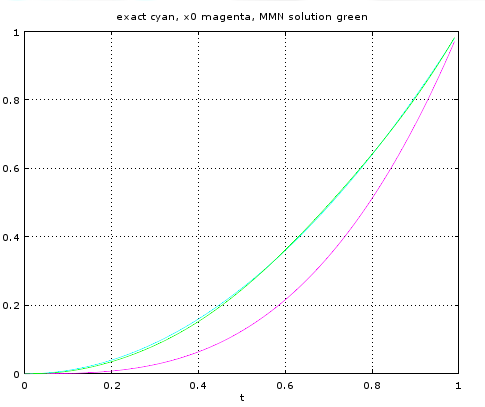
\includegraphics[height=4.0cm]{mmn_ch1}
%	\end{figure}
%	\centering
%	Восстановленное ММН решение.
%\end{frame}
%\begin{frame}{}
%	Точное решение --- функция $z(t)=t^2$, начальное приближение $x^0(t)=t^3$, $\bar\alpha=\alpha=10^{-2}$, критерий останова $\frac{\|x^k-z\|}{\|z\|}\leqslant\varepsilon=10^{-2}$, где $x^k$ --- приближение на $k$-й итерации.
%	$\Delta=\frac{\|F(x^k)+\alpha(x^k-x^0)-y\|}{\|y\|}$ --- относительная норма невязки. 
%	\begin{table}[h]
%		\centering
%		{\scriptsize Табл.1. Результаты для правой части без шума}
%		\begin{tabular}{|l|c|c|c|}
%			\hline
%			\textbf{Метод}                   & \multicolumn{1}{l|}{\textbf{Параметр шага, $\gamma$}} & \multicolumn{1}{l|}{\textbf{$\Delta$}} & \multicolumn{1}{l|}{\textbf{Число итераций, N}} \\ \hline
%			ММО                              & \begin{tabular}[c]{@{}c@{}}0.5\end{tabular}                                       & 0.003                                   & 25                                     \\ \hline
%			\multicolumn{1}{|r|}{ММО модиф.} & 0.5                                                                                                           & 0.003                                   & 22                                     \\ \hline
%			МНС                              & 0.001                                                                                                         & 0.003                                   & 283                                    \\ \hline
%			МНС модиф.                       & \begin{tabular}[c]{@{}c@{}}0.02 (c 0-й итер.), \\ 0.005 (c 30-й итер.),\\   0.002 (c 32-й итер.)\end{tabular} & 0.003                                   & 32                                     \\ \hline
%			ММН                              & 1                                                                                                             & 0.003                                   & 32                                     \\ \hline
%			ММН модиф.                       & 1                                                                                                             & 0.003                                   & 27                                     \\ \hline
%			РМН                              & 1                                                                                                             & 0.003                                   & 26                                     \\ \hline
%			РМН модиф.                       & \begin{tabular}[c]{@{}c@{}}0.75\end{tabular}                                       & 0.003                                   & 6                                      \\ \hline
%		\end{tabular}
%	\end{table}
%\end{frame}
%\begin{frame}{}
%	{\textbf{\color{blue}Цель:}}{\textbf{\color{blue}Цель:}} проверить глобальную сходимость методов для задачи с возмущенной правой частью.
%	
%	$\delta=0.1$, $\|y-y^{\delta}\|=0.07<\delta$. Точное решение --- функция $z(t)=t^2$. Начальное приближение $x^0(t)=0$, $\gamma=1$, $\bar\alpha=1$, $\alpha=10^{-3}$, критерий останова $\frac{\|x^k-z\|}{\|z\|}\leqslant\varepsilon=0.25$, где $x^k$ --- приближение на $k$-й итерации. 
%	\begin{table}[H]
%		\centering
%		{\scriptsize Табл.1. Результаты для задачи с шумом}
%		\begin{tabular}{|l|c|c|}
%			\hline
%			\textbf{Метод}                   & \multicolumn{1}{l|}{\textbf{$\Delta$}} & \multicolumn{1}{l|}{\textbf{Число итераций, N}} \\ \hline
%			ММО                              & 0.042                                  & 9                                               \\ \hline
%			\multicolumn{1}{|r|}{ММО модиф.} & 0.042                                  & 9                                               \\ \hline
%			МНС                              & 0.041                                  & 9                                               \\ \hline
%			МНС модиф.                       & 0.040                                  & 9                                               \\ \hline
%			ММН                              & 0.045                                  & 9                                               \\ \hline
%			ММН модиф.                       & 0.045                                  & 9                                               \\ \hline
%			РМН                              & 0.042                                  & 9                                               \\ \hline
%			РМН модиф.                       & 0.042                                  & 8                                               \\ \hline
%		\end{tabular}
%	\end{table}
%	{\textbf{\color{blue}Вывод:}} удалось достигнуть точности $\varepsilon<\|u^\delta-\hat{u}\|$, относительная норма невязки уменьшается с каждой итерацией.
%\end{frame}
\begin{frame}{Глава 2. Решение уравнений с немонотонным оператором}
	
	Во второй главе показано, что есть возможность ослабить условие монотонности оператора $A$ исходного уравнения и обосновать сходимость итераций РМН, ММО, МНС, ММН в конечномерном случае.
	
	\smallskip
	Представлены доказательства сходимости метода Ньютона, нелинейных $\alpha$-процессов и их модифицированных аналогов, приведены результаты численных расчетов.
\end{frame}
\begin{frame}
%	Цель --- обосновать сходимость рассматриваемых процессов в конечномерном случае, когда оператор $A\colon R^n \to R^n$, для которого матрица $A'(u)$ в некоторой окрестности решения имеет спектр, состоящий из различных неотрицательных собственных значений.
	\begin{block}{\bf Лемма (Васин, 2017)}
		Пусть $n\times n$ матрица $A'(u)$ не имеет кратных собственных значений $\lambda _i$ и числа $\lambda _i$ ($i=1,2,..n$) различны и неотрицательны. Тогда при $\bar\alpha>0$ матрица имеет представление $A'(u)+\bar\alpha I =S(u)\Lambda(u) S^{-1}(u)$ и справедлива оценка
		$$\|(A'(u)+\bar\alpha I)^{-1}\|\leqslant \frac{\mu (S(u))}{\bar\alpha+\lambda_{min}} \leqslant \frac{\mu(S(u))}{\bar\alpha}, \eqno (2.1)$$
		где столбцы матрицы $S(u)$ составлены из собственных векторов матрицы $A'(u)+\bar\alpha I$, $\Lambda$--- диагональная матрица, ее элементы --- собственные значения матрицы $A'(u)+\bar\alpha I$, $$\mu(S(u))=\|S(u)\|\cdot\|S^{-1}(u)\|,$$
		$\mu(S(u))$ --- число обусловленности $S(u)$.
	\end{block}
\end{frame} 
\begin{frame}{\small 2.1. Скорость сходимости РМН с немонотонным оператором}
	\begin{block}{\bf Теорема ~2.1.}
		Пусть выполнены условия леммы, а также: \quad $$\sup\{\mu(S(u)): u\in S_r(u_\alpha)\}\leqslant\bar S <\infty,$$ 
		$$\|A(u)-A(v)\|\leqslant N_1\|u-v\|,\quad
		\|A'(u)-A'(v)\|\leqslant N_2\|u-v\|, \quad \forall u, v \in U,$$
		$$\|A'(u^0)\| \leqslant N_0\leqslant N_1, \quad \|u^0-u_\alpha\| \leqslant r,$$
		
		\smallskip
		{\textbf{\color{blue}$A'(u^0)$ --- симметричная матрица, $0<\alpha\leqslant\bar\alpha$, $\bar\alpha\geqslant 4N_0$, $r\leqslant\alpha/8N_2\bar S$}}.
		
		\smallskip
		Тогда для метода (1.3) справедливо заключение теоремы (1.3), где
		$$\gamma<\frac{\alpha\bar\alpha}{2(N_1+\alpha)^2\bar S^2},
		\quad
		{\gamma}_{opt}=\frac{\alpha\bar\alpha}{4(N_1+\alpha)^2\bar S^2},$$ 
		$$\|u^k-u_\alpha\|\leqslant q^k r, \quad q=\sqrt{1-\frac{\alpha ^2}{16(N_1+\alpha)^2\bar S^2}}.$$
	\end{block}
\end{frame}
%\begin{frame}
%	\begin{block}{\bf Замечание~3.1} При доказательстве теоремы достаточно требовать ограниченность величины $$\sup\{\mu(S(u^k)): u^k \in S_r(u_\alpha)\},$$ где $u^k$ --- итерационные точки метода. Причем, при регулярном правиле останова итераций $k(\delta)$, супремум берется по конечному набору номеров $k\leqslant k(\delta)$, что автоматически влечет ограниченность супремума и выполняются оценки аналогичные оценкам в теореме (2.3) при этих значениях $k$. Кроме того, для модифицированного метода Ньютона, в котором производная $A'(u^0)$ вычисляется в фиксированной точке $u^0$, величина $\mu(S(u^0))=\|S(u^0)\|\cdot\|S^{-1}(u^0)\|=\bar S<\infty$.
%	\end{block}
%\end{frame}
%\begin{frame}{2.2. Нелинейные альфа-процессы}
%	\begin{block}{\bf Теорема ~2.2.}
%		Пусть выполнены условия леммы, $\|A(u)-A(v)\|\leqslant N_1\|u-v\|,$ \quad $\|A'(u)-A'(v)\|\leqslant N_2\|u-v\|,$ \quad $ \forall u, v \in U,$
%		$	\|A'(u^0)\| \leqslant N_0\leqslant N_1, \quad \|u^0-u_\alpha\| \leqslant r,$ 
%%		
%%		\smallskip
%%		при $u \in S_r(u_\alpha)$ матрица $A'(u)$ имеет спектр, состоящий из неотрицательных различных собственных значений, $A'(u^0)$ --- самосопряженный неотрицательно определенный оператор, параметры удовлетворяют условиям: 
%		$$	MMO:\qquad 0<\alpha\leqslant\bar\alpha, \quad r\leqslant\alpha /6\bar SN_2, \quad \bar\alpha \geqslant N_0 $$
%		$$	MHC:\qquad 0<\alpha\leqslant\bar\alpha, \quad r\leqslant\alpha /3N_2,$$
%		$$	MMH:\qquad 0<\alpha\leqslant\bar\alpha, \quad r\leqslant\alpha /6N_2.$$
%%		Тогда для оператора поправки $$F^\varkappa(u)=\frac{\langle(A'(u^k)+\bar\alpha I)^{\varkappa}S_\alpha(u^k), S_\alpha(u^k)\rangle}{\langle(A'(u^k)+\bar\alpha I)^{\varkappa+1}S_\alpha(u^k), S_\alpha(u^k)\rangle}S_\alpha(u^k)$$
%		справедливо соотношение
%		$$\|F^\varkappa(u)\|^2 \leqslant \mu_\varkappa\langle F^\varkappa(u), u-u_\alpha\rangle, \quad \varkappa=-1,0,1,$$ где
%		$$\mu _{-1}=\frac{8\bar S^2(N_1+\alpha)^2}{\alpha\bar\alpha}, \quad 
%		\mu _0=\frac{18(N_1+\alpha)^2(N_1+\bar\alpha)}{\alpha\bar\alpha ^2}, \quad $$
%		$$\mu _1=\frac{18(N_1+\alpha)^2(N_1+\bar\alpha)^4}{\alpha\bar\alpha ^5}.$$
%	\end{block}
%\end{frame}
\begin{frame}{\small 2.2. Скорость сходимости $\alpha$-процессов с немонотонным оператором}
	\begin{block}{\bf Теорема ~2.2.}
		Пусть выполнены условия леммы. 
		
		Тогда при $\gamma_\varkappa<2/\mu _\varkappa$, $\varkappa=-1,0,1$, с соответствующими $\mu _k$, последовательности ${u^k}$, порождаемые процессом (1.6) при $\varkappa=-1,0,1$, сходятся к $u_\alpha$, т.е., $$\lim_{k\to\infty}\|u^k-u_\alpha\|=0,$$ а при $
		\gamma{_\varkappa^{opt}}=\frac{1}{\mu_\varkappa}$
		справедлива оценка $$\|u^{k+1}-u_\alpha\|\leqslant q{_\varkappa^k}r,$$ где
		$$q_{-1}=\sqrt{1-\frac{\alpha^2}{64\bar S^2(N_1+\alpha)^2}}, \quad q_0=\sqrt{1-\frac{\alpha^2\bar\alpha^2}{36(N_1+\alpha)^2(N_1+\bar\alpha)^2}},$$
		$$q_1=\sqrt{1-\frac{\alpha^2\bar\alpha^6}{36(N_1+\alpha)^2(N_1+\bar\alpha)^6}}.$$
	\end{block}
\end{frame}
%\begin{frame}{\small\textbf{Модифицированные методы на основе нелинейных альфа-процессов}}
%	\begin{block}{Теорема 2.4}
%		Пусть выполнены условия $$\|A(u)-A(v)\|\leqslant N_1\|u-v\|,  \quad \forall u, v \in U,$$ 
%		$$\|A'(u)-A'(v)\|\leqslant N_2\|u-v\|, \quad \forall u, v \in U,$$
%		$$\|A'(u^0)\| \leqslant N_0\leqslant N_1, \quad \|u^0-u_\alpha\| \leqslant r,$$ 
%		
%		\smallskip
%		$A'(u^0)$ --- самосопряженный оператор, спектр которого состоит из неотрицательных различных собственных значений, параметры удовлетворяют условиям:
%		$$0\leqslant\alpha\leqslant\bar{\alpha}, \quad r=\alpha/6N_2, \quad \bar{\alpha}\geqslant N_0.$$
%		
%%		Тогда для оператора поправки на итерации
%%		$$F^\varkappa(u)=\frac{\langle(A'(u^0)+\bar\alpha I)^{\varkappa}S_\alpha(u^k), S_\alpha(u^k)\rangle}{\langle(A'(u^0)+\bar\alpha I)^{\varkappa+1}S_\alpha(u^k), S_\alpha(u^k)\rangle}S_\alpha(u^k)$$ имеет место неравенство
%		Тогда имеет место неравенство
%		$$\|F^\varkappa(u)\|^2\leqslant\frac{8(N_1+\alpha)^2}{3\alpha\bar{\alpha}}\langle F^\varkappa(u), u-u_\alpha\rangle,$$
%		где $ \quad \varkappa=-1, 0, 1,$ для модифицированных вариантов ММО, МНС и ММН соответственно (см. слайд 13).
%	\end{block}
%\end{frame}
\begin{frame}{\small 2.2. Скорость сходимости $\alpha$-процессов с немонотонным оператором}
	Пусть выполнены условия ($*$):
	$\|A(u)-A(v)\|\leqslant N_1\|u-v\|, \quad \|A'(u)-A'(v)\|\leqslant N_2\|u-v\|, \quad \forall u, v \in U,$
	$\|A'(u^0)\| \leqslant N_0\leqslant N_1, \quad \|u^0-u_\alpha\| \leqslant r,$
	{\textbf{\color{blue}$A'(u^0)$ --- самосопряженный оператор, спектр которого состоит из неотрицательных различных собственных значений}}, 
	$0\leqslant\alpha\leqslant\bar{\alpha}, \quad r=\alpha/6N_2, \quad \bar{\alpha}\geqslant N_0.$
			
	\begin{block}{Теорема 2.3}
		Пусть выполнены условия ($*$). Тогда при
		$$\gamma _\varkappa <\frac{2}{\mu _\varkappa}\quad (\varkappa=-1,0,1)$$
		для последовательности $\{u^k\}$, порождаемой модифицированным $\alpha$-процессом при соответствующем $\varkappa$, имеет место сходимость $\lim_{k\to\infty}\|u^k-u_\alpha\|=0, $ а при 
		$\gamma{_\varkappa^{opt}}=\frac{1}{\mu_\varkappa}$
		справедлива оценка $$\|u^k-u_\alpha\|\leqslant q{_\varkappa^k}r,$$ где
		$$q^\varkappa=\sqrt{1-\frac{9\alpha^2}{64(N_1+\alpha)^2}}$$
	\end{block}
\end{frame}
\begin{frame}
	\begin{block}{\bf Замечание~2.1} Предложенный подход к получению оценок скорости сходимости итерационных процессов полностью переносится на случай, когда спектр матрицы $A'(u^k)$, состоящий из различных вещественных значений, содержит набор малых по абсолютной величине отрицательных собственных значений. Пусть $\lambda _1$ --- отрицательное собственное значение с наименьшим модулем $|\lambda_1|$ и $\bar\alpha -|\lambda _1|=\bar\alpha _1<\alpha^*$. Тогда оценка 
		$$\|(A'(u)+\bar\alpha I)^{-1}\|\leqslant \frac{\mu (S(u))}{\bar\alpha+\lambda_{min}} \leqslant \frac{\mu(S(u))}{\bar\alpha},$$ 
		трансформируется в неравенство
		$$\|(A'(u^k)+\bar\alpha I)^{-1}\|\leqslant\frac{\mu(S(u^k))}{\bar\alpha^*}\leqslant\frac{\bar S}{\bar\alpha^*}$$
		Все теоремы остаются справедливыми при замене $\bar\alpha$ на $\bar\alpha^*$.
	\end{block}
\end{frame}
\begin{frame}{\small\textbf{2.3. Решение модельной задачи магнитометрии}}
	\begin{equation*}\begin{aligned}
	\left[A(u)\right](x,y)=\Delta J  \bigg\{&\iint_{D} \frac{H}{[(x-x')^2+(y-y')^2+H^2]^{3/2}}dx'dy' \notag\\
	- &\iint_{D} \frac{u(x',y')}{[(x-x')^2+(y-y')^2+u^2(x',y')]^{3/2}}dx'dy' \bigg\}= B_z(x,y,0),
	\end{aligned} \end{equation*}
	где $\Delta J$ --- скачок $z$-компоненты вектора намагниченности, $z=H$ --- асимптотическая плоскость, $ B_z(x,y,0)$ --- функция аномального поля, $z=u(x,y)$ --- искомая функция, описывающая поверхность раздела сред с различными свойствами намагниченности.
	
	\smallskip
	Точное решение уравнения магнитометрии задается формулой \textbf{\color{red}(Акимова, Мисилов, 2014-2016)}
	$$\hat{u}(x,y)=5-2e^{-(x/10-3.5)^6-(y/10-2.5)^6}-3^{-(x/10-5.5)^6-(y/10-4.5)^6},$$
	\textbf{\color{blue}Результаты.} Число обусловленности $\mu(A'_n(u_n^k))\approx 1.8\cdot 10^7$, спектр неотрицательный, состоящий из различных собственных значений, $\bar\alpha=10^{-2}$, $\alpha = 10^{-4}$, $\gamma=1$, $\varepsilon < 10^{-2}$. Итерационные методы сходятся за 4--5 итераций, у модифицированных меньше время счета.
\end{frame}
%\begin{frame}{}
%	\textbf{\color{blue}Цель:} проверить заключения теорем главы 2 на примере решения обратной задачи магнитометрии.
%	Число обусловленности $\mu(A'_n(u_n^k))\approx 1.8\cdot 10^7$, спектр неотрицательный, состоящий из различных собственных значений, $\bar\alpha=10^{-2}$, $\alpha = 10^{-4}$, $\gamma=1$, $\varepsilon < 10^{-2}$
%	
%	\begin{table}
%		\centering
%		{\scriptsize Табл.2. Относительные нормы невязок, числа итераций и времена счета в задаче магнитометрии}
%		
%		\smallskip
%\begin{tabular}{|c|c|c|c|c|}
%\hline
%Методы                    & ММО    & МНС    & ММН    & РМН    \\ \hline
%\multirow{2}{*}{$\Delta$} & 0.0636 & 0.0699 & 0.0802 & 0.0368 \\ \cline{2-5} 
%                          & 0.0569 & 0.0575 & 0.0595 & 0.0369 \\ \hline
%\multirow{2}{*}{N}        & 4      & 4      & 4      & 5      \\ \cline{2-5} 
%                          & 4      & 4      & 4      & 5      \\ \hline
%\multirow{2}{*}{T (сек)}  & 10     & 6      & 6      & 22     \\ \cline{2-5} 
%                          & 5      & 3      & 3      & 3      \\ \hline
%\end{tabular}
%	\end{table}
%	\textbf{\color{blue}Вывод:} число итераций для модифицированных методов больше, чем для немодифицированных, но затраты машинного времени меньше.
%\end{frame}
\begin{frame}{Глава 3. Покомпонентные методы и вычислительные оптимизации для решения обратных структурных задач гравиметрии и магнитометрии}
	В третьей главе предлагаются покомпонентные методы типа Ньютона и Левенберга -- Марквардта и вычислительная оптимизация методов типа Ньютона. 
	
	Параллельные алгоритмы реализованы в виде комплекса программ на многоядерных и графических процессорах (видеокартах) для вычислений на сетках большого размера. Приводятся результаты расчетов на многоядерных процессорах и графических ускорителях. 
	
\end{frame}
\begin{frame}{\small\textbf{3.1. Покомпонентный метод типа Ньютона для обратных задач гравиметрии (new)}}
	Рассмотрим уравнение гравиметрии в декартовой системе координат с осью $z$, направленной вниз 
	\begin{equation*}
	\begin{aligned}
	A(u)=\gamma\Delta\sigma \bigg\{ &\iint_{D} \frac{1}{[(x-x')^2+(y-y')^2+H^2]^{1/2}}dx'dy' \\
	- &\iint_{D} \frac{1}{[(x-x')^2+(y-y')^2+u^2(x',y')]^{1/2}}dx'dy'\bigg\}=\Delta g(x,y),
	\end{aligned} 
	\end{equation*}
	где $\gamma$ --- гравитационная постоянная, равная $6.67\cdot10^{-8}$ см$^3/$г$\cdot c^2$, $\Delta\sigma=\sigma_2-\sigma_1$ --- скачок плотности на поверхности раздела сред, описываемой функцией $u(x,y)$ и подлежащей определению, $\Delta g(x,y)$ --- аномальное гравитационное поле, вызванное отклонением поверхности от асимптотической плоскости $z=H$ для искомого решения $u(x,y)$.
	
	Уравнение задачи магнитометрии приводилось на слайде 26.
\end{frame}

\begin{frame}{\small\textbf{Модель двуслойной среды}}
	\begin{figure}[h]
		\centering
		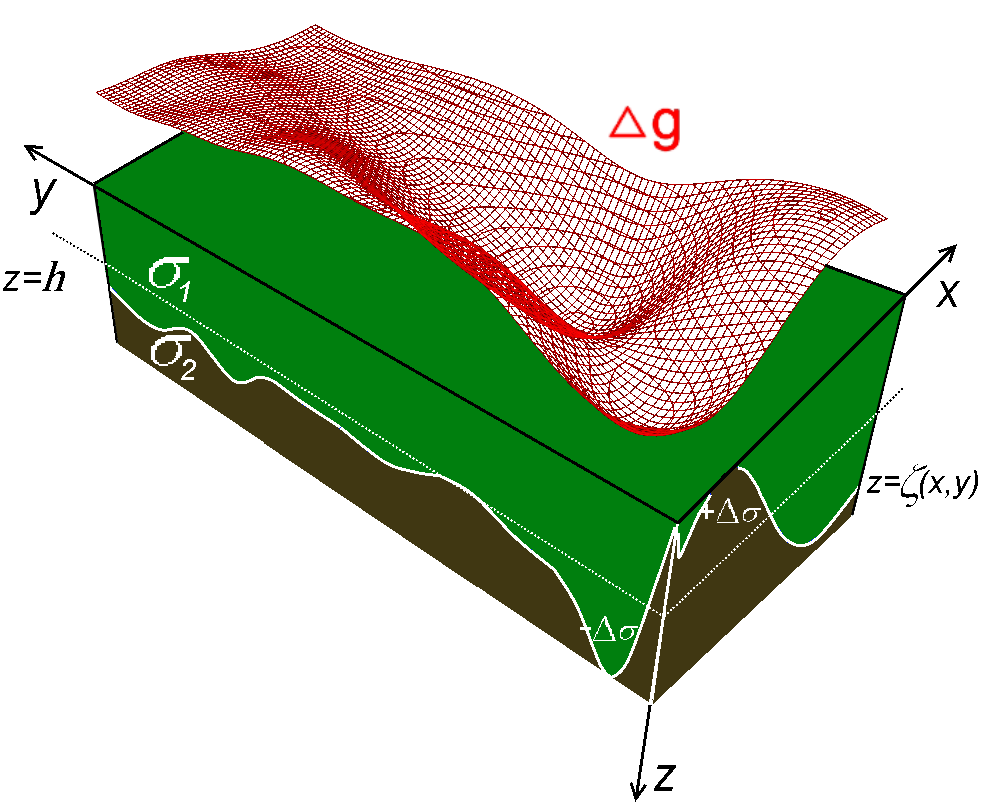
\includegraphics[height=7.0cm]{grav_illust.png}
		\label{fig:twolayer}
	\end{figure}
	\centering
\end{frame}
\begin{frame}{3.1. Покомпонентный метод типа Ньютона (new)}
	Запишем исходное операторное уравнение (1.1) в виде:
	$$P(u)=A(u)-f,$$
	где $A(u)=\int_{a}^{b}\int_{c}^{d}K(x,y, x',y',u^k(x,y))dxdy$ --- интегральный оператор задачи гравиметрии.
	
	Итерации в методе Ньютона строятся по схеме
	$$A'(u^k)(\Delta u^k)=-(A(u^k)-f),$$ где $\Delta u^k=u^{k+1}-u^k$.
	Для задачи гравиметрии
	$$f\Delta\sigma\int_{a}^{b}\int_{c}^{d}K'_u(x,y, x',y',u^k(x,y))\Delta u^k dxdy=A(u(x',y'))-f(x',y').$$
\end{frame}
\begin{frame}{}
	В задаче гравиметрии {\textbf{\color{blue}на изменение гравитационного поля в правой части наибольшее значение оказывает отклонение от асимптотической плоскости в точке $(x',y')$}}. Тогда можем записать
	$$f\Delta\sigma(\Delta u^k)\int_{a}^{b}\int_{c}^{d}K'_u(x,y, x',y',u^k(x,y)) dxdy=A(u(x',y'))-f(x',y').$$
	Итерации осуществляются по схеме:
	$$u^{k+1}(x',y')=u^k(x',y')-\gamma\frac{1}{\varPsi(x',y')}([A(u^k)](x',y')-f(x',y')),$$
	где $$\varPsi(x',y')=f\Delta\sigma\int_{a}^{b}\int_{c}^{d}K'_u(x,y, x',y',u^k(x,y)) dxdy.$$
	Регуляризованный вариант:
	$$u^{k+1}(x',y')=u^k(x',y')-\frac{1}{\varPsi(x',y')+\bar{\alpha}}([A(u^k)](x',y')+\alpha (u(x',y')-u^0(x',y'))-f_\delta(x',y')),$$
	где $\alpha, \bar{\alpha}$ --- положительные параметры регуляризации.
	\let\thefootnote\relax\let\thefootnote\relax\footnotetext{\footnotesize Akimova E., Skurydina A. A componentwise Newton type method for solving the structural inverse gravity problem // EAGE Geoinformatics 2015 – 14th Intern. Conference on Geoinformatics. Kiev, Ukraine. 11–14 May 2015}
\end{frame}
\begin{frame}{\small\textbf{3.2. Оптимизация метода Ньютона для задач гравиметрии и магнитометрии}}
	Прозводная оператора $A$ в точке $u^0(x,y)$ определяется формулой:
	\begin{itemize}
		\item в задаче гравиметрии
		$$ [A'(u^0)]h=\iint_{D} \frac{u^0(x',y')h(x',y')}{[(x-x')^2+(y-y')^2+(u^0(x',y'))^2]^{3/2}}dx'dy',$$
		\item в задаче магнитометрии
		$$ [A'(u^0)]h=\iint_{D} \frac{(x-x')^2+(y-y')^2-2(u^0(x',y'))^2}{[(x-x')^2+(y-y')^2+(u^0(x',y'))^2]^{5/2}}h(x',y')dx'dy'.$$
	\end{itemize}

\begin{block}{Замечание 3.1.}
	В структурных обратных задачах грави- магнитометрии при решении методом Ньютона без существенной потери точности можно не учитывать значения элементов, отстоящих от диагонали далее, чем на  $\beta$-ю часть  размерности матрицы производной.
\end{block}
\let\thefootnote\relax\let\thefootnote\relax\footnotetext{\footnotesize Akimova E., Miniakhmetova A., Martyshko M. Optimization and parallelization of Newton type methods for solving structurial gravimetry and magnetometry inverse problems // EAGE Geoinformatics 2014 – 13th Intern. Conference on Geoinformatics. Kiev, Ukraine. 12–15 May 2014}
\end{frame}
%\begin{frame}
%	\begin{block}{Замечание 3.1.}
%		В структурных обратных задачах грави- магнитометрии при решении методом Ньютона без существенной потери точности можно не учитывать значения элементов, отстоящих от диагонали далее, чем на  $\beta$-ю часть  размерности матрицы производной, то есть те значения $a_{ij}$, для которых  $j \in \{i-h(\beta),..i+h(\beta)\} $, где $h(\beta)$ --- полуширина ленты матрицы, $i, j$ --- индекс элемента.
%	\end{block}
%	\let\thefootnote\relax\let\thefootnote\relax\footnotetext{\footnotesize Akimova E., Miniakhmetova A., Martyshko M. Optimization and parallelization of Newton type methods for solving structurial gravimetry and magnetometry inverse problems // EAGE Geoinformatics 2014 – 13th Intern. Conference on Geoinformatics – Theoretical and Applied Aspects. Kiev, Ukraine. 12–15 May 2014}
%\end{frame}
%\begin{frame}{\small\textbf{Регуляризованный метод Левенберга -- Марквардта (Васин В.В.)}}
%	Регуляризованный метод Левенберга -- Марквардта \textbf{\color{red}(Васин, 2012)}
%	\begin{equation}\label{LM_Vasin}
%	u^{k+1}=u^k-\gamma[A'(u^k)^*A'(u^k)+\alpha I]^{-1} [A'(u^k)^*(A(u^k)-f_\delta)]
%	\end{equation} и его модифицированный вариант \textbf{\color{red}(Васин, Пересторонина, 2011)}
%	\begin{equation}\label{LM_modif_Vasin}
%	u^{k+1}=u^k-\gamma[A'(u^0)^*A'(u^0)+\alpha I]^{-1} [A'(u^k)^*(A(u^k)-f_\delta)]
%	\end{equation}
%	где $\gamma$ --- демпфирующий множитель, $u^0$ --- некоторое приближение к $u_\alpha$, $\alpha>0$.
%\end{frame}
\begin{frame}{Модель многослойной среды}
	\begin{figure}[h]
		\centering
		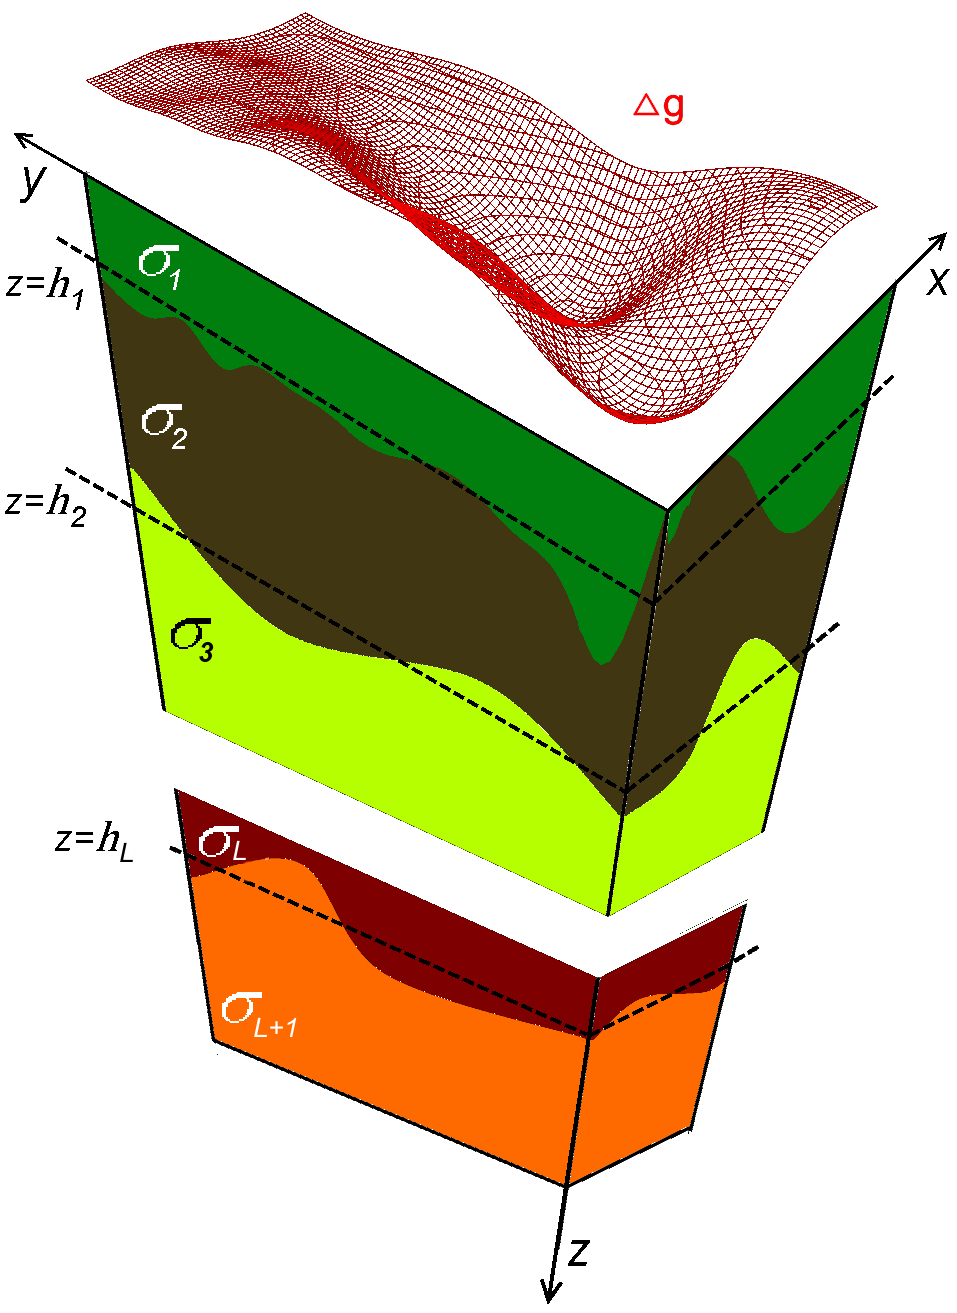
\includegraphics[height=7.0cm]{whitegrav.png}
		\label{fig:multlayer}
	\end{figure}
	\centering
	%Рис.3. Модель многослойной среды.
\end{frame}
\begin{frame}{Постановка задачи}
	Суммарное гравитационное поле получаем путем сложения гравитационных полей от каждой поверхности:
	\begin{equation*}
	\begin{aligned}
	A(u)=\sum_{l=1}^{L}f\Delta\sigma_l\frac{1}{4\pi}\iint_D\bigg\{\frac{1}{[(x-x')^2+(y-y')^2+u_l^2(x,y)]^{1/2}} \\
	-\frac{1}{[(x-x')^2+(y-y')^2+H_l^2]^{1/2}}\bigg\}=\Delta g(x',y'),
	\end{aligned}
	\end{equation*}
	где $L$~--- число границ раздела.
\end{frame}
\begin{frame}{\small\textbf{3.3. Покомпонентный метод типа Левенберга Марквардта для решения задач гравиметрии для модели многослойной среды \textbf{(new)}}}
	По аналогии с покомпонентным методом Ньютона предложен покомпонентный метод типа Левенберга -- Марквардта:
	\begin{equation}\label{comp_lm_meth}
	u_l^{k+1}=u_l^k-\gamma\frac{1}{\varphi_l+\bar{\alpha}}\Lambda[ A'(u_l^k)^T(A(u^k)-f_\delta)],
	\end{equation}
	где $l$ --- номер границы раздела, $l=1,..,L$, $\Lambda$ --- весовой оператор, 
	\begin{equation*}
	\begin{aligned}
	\varphi_l=\bigg[ f\Delta\sigma\int_{a}^{b}\int_{c}^{d}
	K'_u(x',y', x, y, u_l^k(x',y'))dydx\bigg] \notag \\ \times\bigg[f\Delta\sigma\int_{a}^{b}\int_{c}^{d}K'_u(x,y, x',y',u_l^k(x,y))dxdy\bigg]. 
	\end{aligned}
	\end{equation*} 
	где $K'_u(x',y', x, y, u_l^k(x',y'))$ --- ядро интегрального оператора. %транспонированного к ядру $K'_u(x,y,$ $ x',y',u^k(x,y))$.
	 Величина $\varphi_l$ зависит от $u_l^k$.
	\let\thefootnote\relax\let\thefootnote\relax\footnotetext{\tiny Skurydina A. F. Regularized Levenberg –- Marquardt Type Method Applied to the Structural Inverse Gravity Problem in a Multilayer Medium and its Parallel Realization // Bulletin of South Ural State University. Series: Computational Mathematics and Software Engineering. V.6, N.3. pp. 5--15}

\end{frame}
\begin{frame}
	Перепишем в дискретной форме
	\begin{equation}\label{comp_lm_meth_disc}
	u_{l,i}^{k+1}=u_{l,i}^k-\gamma\frac{1}{\varphi_{l,i}+\bar{\alpha}}w_{l,i}\bigg[ \{A'(u_l^k)^T(A(u^k)-f_\delta)\}_i\bigg],
	\end{equation}
	где $w_{l,i}$ --- $i$-й весовой множитель, зависящий от $l$-й границы раздела \textbf{\color{red}(Акимова, Мисилов 2015)},
	\begin{equation*}
	\begin{aligned}
	\varphi_{l,i}=\bigg[ f\Delta\sigma\sum\limits_{k=1}^{N}
	\sum\limits_{m=1}^{M}
	K'_u(x'_k,y'_m, \{x, y\}_i, u_{l,i}^k) \Delta x' \Delta y'\bigg] \notag \\ \times\bigg[f\Delta\sigma\sum\limits_{k=1}^{N}
	\sum\limits_{m=1}^{M}K'_u(x_k,y_m, \{x',y'\}_i,u_l^k(x_k,y_m))\Delta x \Delta y\bigg]. 
	\end{aligned}
	\end{equation*}
	\let\thefootnote\relax\let\thefootnote\relax\footnotetext{\footnotesize Акимова, Е. Н., Мисилов, В. Е., Скурыдина, А. Ф., Третьяков, А. И. Градиентные методы решения структурных обратных задач гравиметрии и магнитометрии на суперкомпьютере “Уран” // Вычислительные методы и программирование, 2015. Т. 16, 155–164.}
\end{frame}
%\begin{frame}{\small\textbf{Приложения к обратным задачам гравиметрии и магнитометрии}}
%	Уравнение гравиметрии в декартовой системе координат с осью $z$, направленной вниз 
%	\begin{equation*}
%	\begin{aligned}
%	A(u)=\gamma\Delta\sigma \bigg\{ &\iint_{D} \frac{1}{[(x-x')^2+(y-y')^2+H^2]^{1/2}}dx'dy' \notag\\
%	- &\iint_{D} \frac{1}{[(x-x')^2+(y-y')^2+u^2(x',y')]^{1/2}}dx'dy'\bigg\}=\Delta g(x,y),
%	\end{aligned} 
%	\end{equation*}
%	Уравнение магнитометрии имеет вид
%	\begin{equation*}\begin{aligned}
%	A(u)=\Delta J  \bigg\{&\iint_{D} \frac{H}{[(x-x')^2+(y-y')^2+H^2]^{3/2}}dx'dy' \notag\\
%	- &\iint_{D} \frac{u(x',y')}{[(x-x')^2+(y-y')^2+u^2(x',y')]^{3/2}}dx'dy' \bigg\}=\Delta G(x,y),
%	\end{aligned} \end{equation*}
%\end{frame}
%\begin{frame}{Задача 1}
%	Точное решение уравнения гравиметрии, определяющее поверхность раздела сред, задается формулой %\textbf{\color{red}(Акимова, Мисилов, Скурыдина, Третьяков, 2015)}
%	\begin{equation*}
%	\hat{u}(x,y)=5-2e^{-(x/10-3.5)^6-(y/10-2.5)^6}-3e^{-(x/10-5.5)^6-(y/10-4.5)^6},
%	\end{equation*}
%	\begin{center}
%		
%		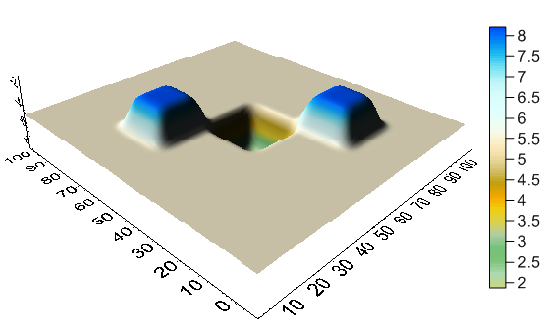
\includegraphics[width=7cm, height=4 cm]{Gravy_exact.png}            %frame~2
%	\end{center}
%	
%	\begin{center}
%		Рис.2. Модельная поверхность: $D=\{0\leqslant x\leqslant 100, \,\,0\leqslant y\leqslant 110\}$, \\ $  H=5,\,\,\Delta x=\Delta y=1,\,\,\Delta\sigma=0.21$г/см$^3$.
%	\end{center}
%\end{frame}
%\begin{frame}{\small\textbf{Результаты численных расчетов в задаче гравиметрии}}
%	Число обусловленности $\mu(A'_n(u_n^k))\approx 4.8 * 10^{8}$, спектр неотрицательный, собственные значения различны. Правило выхода из процесса итераций каждого из методов
%	$$\frac{\|\hat{u}_n-\tilde{u}_n\|_{R^n}}{\|\tilde{u}_n\|_{R^n}}\leqslant 10^{-2},$$
%	где $\hat{u}_n$ --- точное решение, а $\tilde{u}_n$ --- восстановленное каждым из четырех итерационных методов. Таким образом, точность численного решения, полученного методом Ньютона, $\alpha$-процессамии их модифицированными аналогами, гарантированно не превышала $\varepsilon=10^{-2}$.
%\end{frame}
%\begin{frame}
%	При значениях параметров $\bar\alpha=\alpha=10^{-3}$, $\gamma=1$ представлены результаты численных расчетов, где
%	$$\Delta=\frac{\|A_n(\tilde{u}_n)+\alpha(\tilde{u}_n-u^0)-f_n\|_{R^n}}{\|f_n\|_{R^n}},$$
%	$N$ --- число итераций в процессе для достижения точности $10^{-2}$, $T$ --- время реализации метода. В позициях для $\Delta$, $N$, $T$ верхняя строка соответствует основным процессам, а нижняя --- их модифицированным вариантам.
%	\begin{table}
%		\centering
%		{\scriptsize Табл.1. Относительные нормы невязок, итерации и времена счета в задаче гравиметрии}
%		
%		\begin{tabular}{|p{0.25\textwidth}|p{0.1\textwidth}|p{0.1\textwidth}|p{0.1\textwidth}|p{0.1\textwidth}|}
%			\hline
%			\rule{0cm}{0.5cm}
%			Методы & ММО & МНС & ММН & РМН \\ \hline
%			\rule{0cm}{0.5cm}
%			\multirow{$\Delta$} & 0.0048 & 0.0020 & 0.0024 & 0.0023	 \\ \cline{2-5} 
%			\rule{0cm}{0.5cm}
%			&  0.0094   & 0.0019    &  0.0019   &  0.0021   \\ \hline
%			\rule{0cm}{0.5cm}
%			\multirow{$N$} & 17  &  21   &   20  &  16    \\ \cline{2-5}
%			\rule{0cm}{0.5cm}
%			&  22   &   23  &  23   &  16   \\ \hline
%			\rule{0cm}{0.5cm}
%			\multirow{$T$ (сек)}    &  20   &  11   &  14  & 16    \\ \cline{2-5}
%			\rule{0cm}{0.5cm}
%			& 25    & 8    &  8   &   8  \\ \hline
%		\end{tabular}
%	\end{table}
%\end{frame}

\begin{frame}{3.4. Описание комплекса параллельных программ}
	\begin{itemize}
		\item на основе предложенных методов разработаны параллельные алгоритмы для вычислений на многоядерных процессорах и графических ускорителей;
		\item используются инструменты: OpenMP, CUDA;
		\item библиотеки Intel MKL, Cublas;
		\item при больших размерах сеток вычисления производились <<на лету>>: необходимый элемент матрицы вычисляется в момент умножения его на элемент вектора.
	\end{itemize}
	
	Для оценки производительности параллельных алгоритмов используются показатели {\textbf{ускорения и эффективности}}
	$$
	S_m=\frac{T_1}{T_m},\quad
	\quad E_m=\frac{S_m}{m}, $$
	где $T_1$ --- время выполнения последовательного алгоритма,
	$T_m$ --- время выполнения параллельного алгоритма на $m$ ($m>1$) ядрах процессора.
\end{frame}
\begin{frame}{Технология OpenMP}
	\begin{figure}[h]
		\centering
		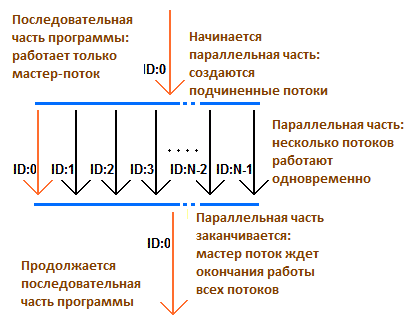
\includegraphics[width=0.6\textwidth]{omp}
	\end{figure}
	\centering
	Принцип работы потоков в OpenMP.
\end{frame}
\begin{frame}{Технология CUDA}
	\begin{figure}[h]
		\centering
		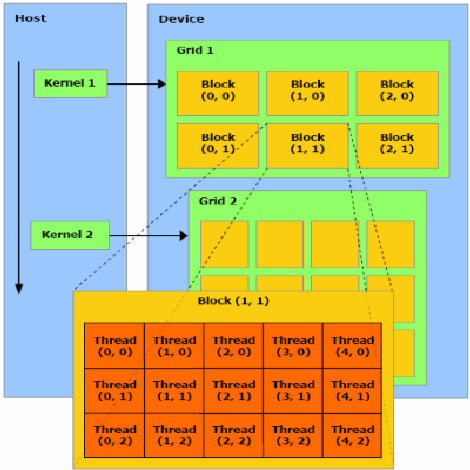
\includegraphics[width=0.6\textwidth]{cuda}
	\end{figure}
	\centering
	Иерархия компонентов вычислительной сетки GPU.
\end{frame}
\begin{frame}{\small 3.5. Задача 1 (сравнение методов типа Ньютона при решении обратной задачи гравиметрии для двухслойной среды)}
	%\textbf{\color{blue}Цель:} решить обратную задачу гравиметрии методами типа Ньютона с распараллеливанием OpenMP.
	
	Точное решение уравнения гравиметрии, определяющее поверхность раздела сред, задается формулой
	$$\hat{u}(x,y)=5+4e^{-(x/10-3.5)^4-(y/10-2.5)^4}-3e^{-(x/10-5.5)^4-(y/10-4.5)^4},$$
	\centering
		
	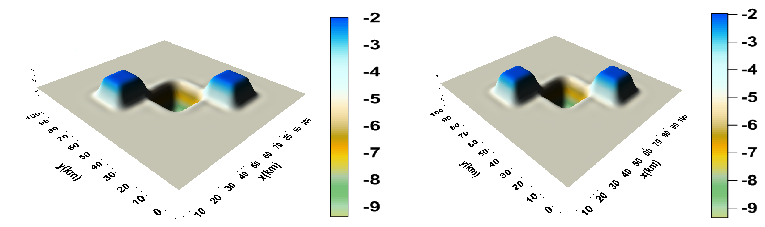
\includegraphics[width=\textwidth, height=0.35\textheight]{gravy_kiev2014.png}
	
	Модельная поверхность (слева) и приближенное решение (справа): $D=\{0\leqslant x\leqslant 270, \,\,0\leqslant y\leqslant 300\}$, \\ $  H=5,\,\,\Delta x=\Delta y=1,\,\,\Delta\sigma=0.2$ г/см$^3$.
\end{frame}
\begin{frame}
	Критерий останова итераций 
	$\delta=\frac{\|u_e-u_a\|}{\|u_e\|}\leqslant 0.025,$ параметр регуляризации $\alpha=\bar{\alpha}=10^{-3}$, полуширина ленты матрицы производной $\beta=1/4$ для задачи гравиметрии. Коэффициент $\gamma=1.2$ для покомпонетного метода Ньютона, $\Delta=\|A(u^k)+\alpha(u^k-u^0)-f_\delta\|/\|f_\delta\|$
	
	\begin{table}[]
		\centering
		\renewcommand{\arraystretch}{1.5}
		\scriptsize{Табл.3. Сравнение методов решения задачи гравиметрии}
		\label{table3.1}
		\begin{tabular}{|p{0.3\textwidth}|p{0.05\textwidth}|l|l|l|l|l|}
			\hline
			\multicolumn{1}{|c|}{Метод}        & \multicolumn{1}{c|}{$N$} &
			\multicolumn{1}{c|}{$\Delta$} & \multicolumn{1}{c|}{$T_1$} & \multicolumn{1}{c|}{$T_8$} &
			\multicolumn{1}{c|}{$S_8$} & \multicolumn{1}{c|}{$E_8$}
			\\ \hline
			Метод Ньютона                      &  3        & 0.041                          &       22 мин                  &     2 мин 40 сек &
			8 & 1 \\ \hline
			Модифицированный метод Ньютона     &         5           & 0.042            & 32 мин                  & 4 мин      &
			8 & 1             \\ \hline
			Метод Ньютона с ленточной матрицей &  4               & 0.041                    & 24 мин                  & 3 мин       & 8 & 1            \\ \hline
			\rowcolor{Green}
			Покомпонентный метод Ньютона &  6               & 0.041                    & 17 мин                  & 2 мин       & 8 & 1            \\ \hline
		\end{tabular}
	\end{table}
	\textbf{\color{blue}Вывод:} покомпонентный метод типа Ньютона является самым экономичным по вычислительным затратам. Исключение из матрицы производной оператора элементов практически не влияет на сходимость метода Ньютона. 
\end{frame}
%\begin{frame}
%	Точное решение уравнения магнитометрии, определяющее поверхность раздела сред, задается формулой
%	$$\hat{u}(x,y)=5-2e^{-(x/10-3.5)^6-(y/10-2.5)^6}-3e^{-(x/10-5.5)^6-(y/10-4.5)^6},$$
%	\centering
%	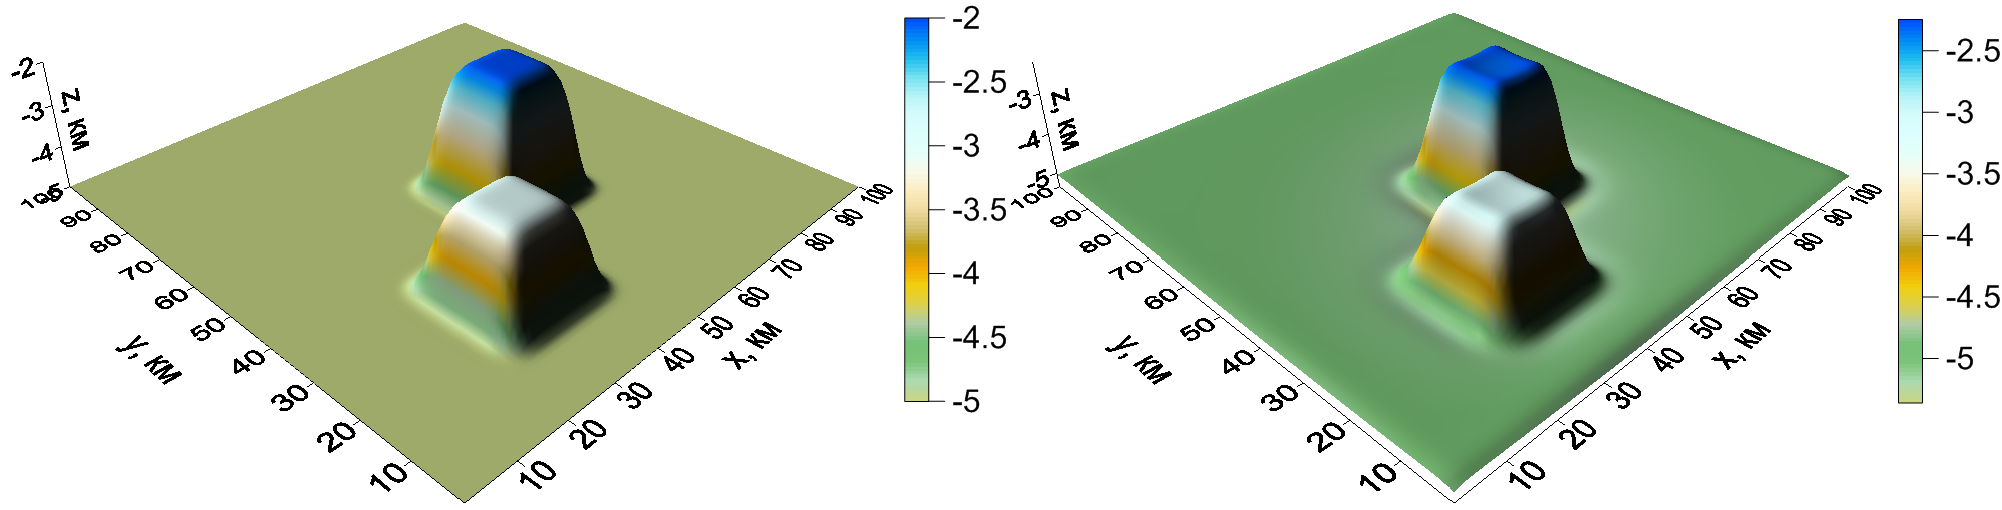
\includegraphics[width=\textwidth, height=0.3\textheight]{magne_kiev2014.png}
%	
%	Рис.5. Модельная поверхность (слева) и приближенное решение (справа): $D=\{0\leqslant x\leqslant 300, \,\,0\leqslant y\leqslant 300\}$, \\ $  H=5,\,\,\Delta x=\Delta y=0.3,\,\,\Delta J=0.4$ А/м.
%\end{frame}
%\begin{frame}
%	В таблице приведены результаты расчетов, критерий останова итераций 
%	$$\delta=\frac{\|u_e-u_a\|}{\|u_e\|}\leqslant 0.025,$$ параметр регуляризации $\alpha=\bar{\alpha}=10^{-3}$, полуширина ленты матрицы производной $\beta=1/5$ для задачи магнитометрии.
%	\begin{table}[]
%		\centering
%		{\scriptsize Табл.4. Решение обратной задачи магнитометрии в двухслойной среде}
%		\begin{tabular}{|p{0.25\textwidth}|p{0.05\textwidth}|l|l|l|l|l|}
%			\hline
%			\multicolumn{1}{|c|}{Метод}        & \multicolumn{1}{c|}{$N$} &
%			\multicolumn{1}{c|}{$\Delta$} &
%			\multicolumn{1}{c|}{$T_1$} & \multicolumn{1}{c|}{$T_8$} &	\multicolumn{1}{c|}{$S_8$}&\multicolumn{1}{c|}{$E_8$} \\ \hline
%			Метод Ньютона                      &   3             & 0.05                  &     9 мин                   &      1 мин 30 сек   
%			& 6 &        0.75     \\ \hline
%			Модифицированный метод Ньютона     &              6           & 0.051           & 15 мин 30 сек                & 2 мин  & 7.75 & 0.96\\ \hline
%			Метод Ньютона с ленточной матрицей &   5                    & 0.05               & 9 мин 36 сек    & 1 мин 12 сек & 8 & 1   \\ \hline
%		\end{tabular}
%	\end{table}
%	{\bfseries \large Вывод.} Исключение из матрицы производной оператора $A'(u^k)$ элементов, далеко отстоящих от диагонали, почти не влияет на сходимость метода Ньютона.
%\end{frame}

\begin{frame}{\small 3.5. Задача 2 (сравнение методов типа Ньютона на больших сетках)}
	%\textbf{\color{blue}Цель:} Решить задачу гравиметрии и сравнить модифицированный метод Ньютона и покомпонентный метод Ньютона на больших сетках.
	
	Точное решение уравнения гравиметрии, определяющее поверхность раздела сред, задается формулой
	\begin{equation*}
	\begin{aligned}
	\hat{u}(x,y)=5-3.21e^{-(x/10.13-6.62)^6-(y/9.59-2.93)^6}-2.78e^{-(x/9.89-4.12)^6-(y/8.63-7.435)^6}\\+3.19e^{-(x/9.89-4.82)^6-(y/8.72-4.335)^6},
	\end{aligned} 
	\end{equation*}
%	\centering
%	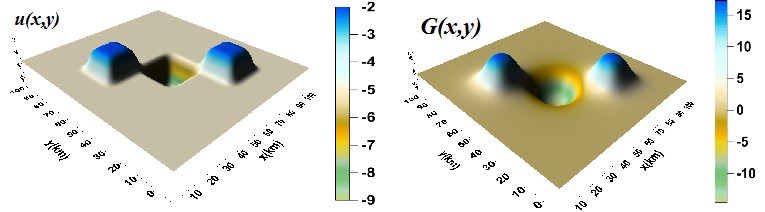
\includegraphics[width=\textwidth, height=0.35\textheight]{gravy_kiev2015.png}
%	
%	Рис.6. Модельная поверхность (слева) и синтетическое гравитационное поле (справа): $D=\{0\leqslant x\leqslant 300, \,\,0\leqslant y\leqslant 330\}$, \\ $  H=5,\,\,\Delta x=\Delta y=0.33,\,\,\Delta\sigma=0.21$ г/см$^3$.
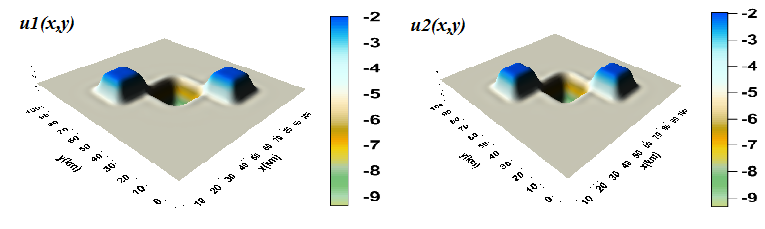
\includegraphics[width=\textwidth, height=0.35\textheight]{gravy_kiev2015_methods.png}

\centering
Решение, полученное модиф. методом Ньютона (слева) и решение, полученное покомпонентным методом (справа).

\end{frame}
%\begin{frame}
%	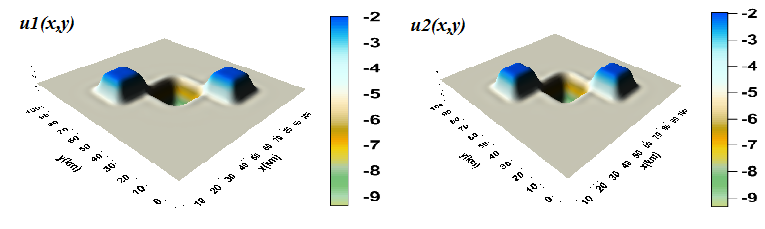
\includegraphics[width=\textwidth, height=0.35\textheight]{gravy_kiev2015_methods.png}
%	
%	\centering
%	Рис.7. Решение, полученное модиф. методом Ньютона (слева) и решение, полученное покомпонентным методом (справа).
%	
%	\flushleft
%	1. Параметр регуляризации взят $\alpha=\bar{\alpha}=10^{-3}$,
%	
%	2. Демпфирующий параметр $\gamma=1.8$ для покомпонентного метода Ньютона.
%	
%	Критерий останова итераций $$\varepsilon=\frac{\|u_e-u_a\|}{\|u_e\|}=10^{-2}.$$
%\end{frame}
\begin{frame}
	Параметры регуляризации $\alpha=\bar{\alpha}=10^{-3}$, $\gamma=1.8$ для покомпонентного метода Ньютона, критерий останова $\varepsilon=\frac{\|u_e-u_a\|}{\|u_e\|}=10^{-2}.$
	\begin{table}[]
		\centering
		{\scriptsize Табл.5. Сравнение ММН и ПМН}
		\begin{tabular}{|l|c|c|}
			\hline
			\textbf{Показатели}                                                        & \multicolumn{1}{l|}{\textbf{\begin{tabular}[c]{@{}l@{}}Модифицированный\\ метод Ньютона\end{tabular}}} & \multicolumn{1}{l|}{\textbf{\begin{tabular}[c]{@{}l@{}}Покомпонентный\\ метод типа Ньютона\end{tabular}}} \\ \hline
			\begin{tabular}[c]{@{}l@{}}Число итераций,\\ $N$\end{tabular}              & 16                                                                                                     & 21                                                                                                        \\ \hline
			\begin{tabular}[c]{@{}l@{}}Отн. норма\\ невязки, $\Delta$\end{tabular}     & 0.002                                                                                                  & 0.002                                                                                                                                                                                                       \\ \hline
			\rowcolor{Green}
			\textbf{\begin{tabular}[c]{@{}l@{}}Время, $T_1$ \\ на сетке 512$\times$512\end{tabular}} & \textbf{61 мин}                                                                                        & \textbf{19 мин}                                                                                           \\ \hline
			\textbf{\begin{tabular}[c]{@{}l@{}}Время, $T_8$ \\ на сетке 512$\times$512\end{tabular}} & \textbf{7 мин 50 сек}                                                                                  & \textbf{2 мин 33 сек}                                                                                     \\ \hline
			Ускорение, $S_8$                                                                      & 7.82                                                                                                   & 7.45                                                                                                      \\ \hline
			Эффективность, $E_8$                                                                      & 0.97                                                                                                   & 0.93                                                                                                      \\ \hline    
		\end{tabular}
	\end{table}
	{\textcolor{blue}{Вывод.}} Покомпонентный метод Ньютона снижает время решения задачи в три раза по сравнению с модифицированным методом Ньютона. Разработанные параллельные алгоритмы демонстрируют высокую эффективность.
	%Проведенные эксперименты наглядно демонстрируют выгоду использования покомпонентного метода Ньютона для решения обратных задач на больших сетках.
\end{frame}

\begin{frame}{\small 3.5. Задача 3 (методы типа Левенберга -- Марквардта для решения задачи гравиметрии для многослойной среды}
%	\textcolor{blue}{Цель:} сравнить по точности решения и по машинным затратам регуляризованный Левенберга -- Марквардта и покомпонентный типа Левенберга -- Марквардта.
	\begin{figure}
		\centering
		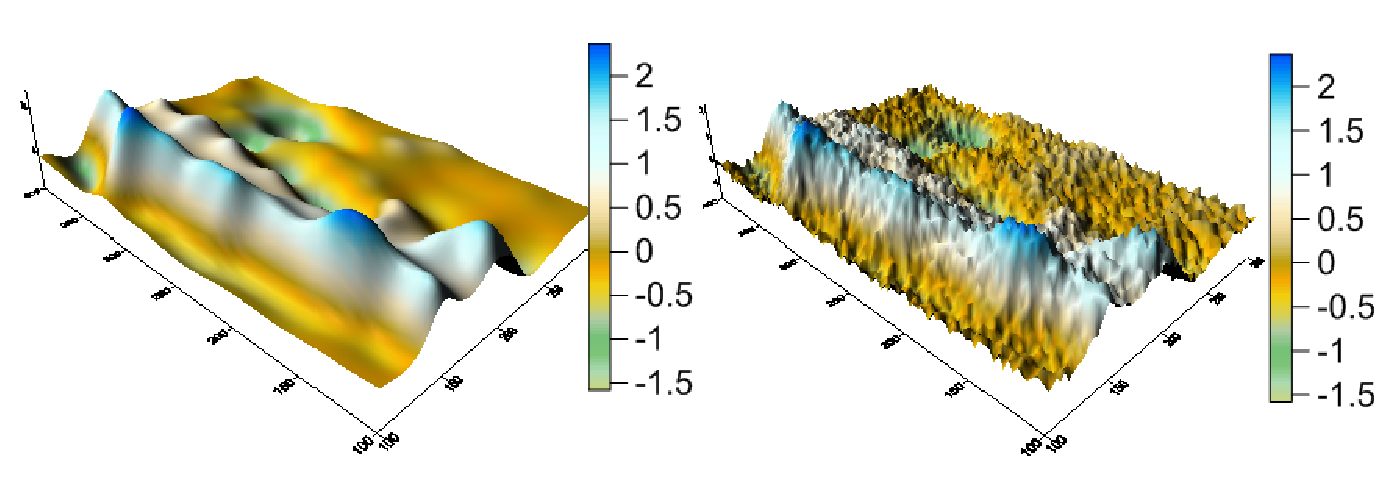
\includegraphics[height=0.2\textheight]{fields}
		
		\centering\textit{Суммарное поле и поле с шумом 22\% (мГал), $\mu=1$, $\sigma=1.15$.}
		\centering
		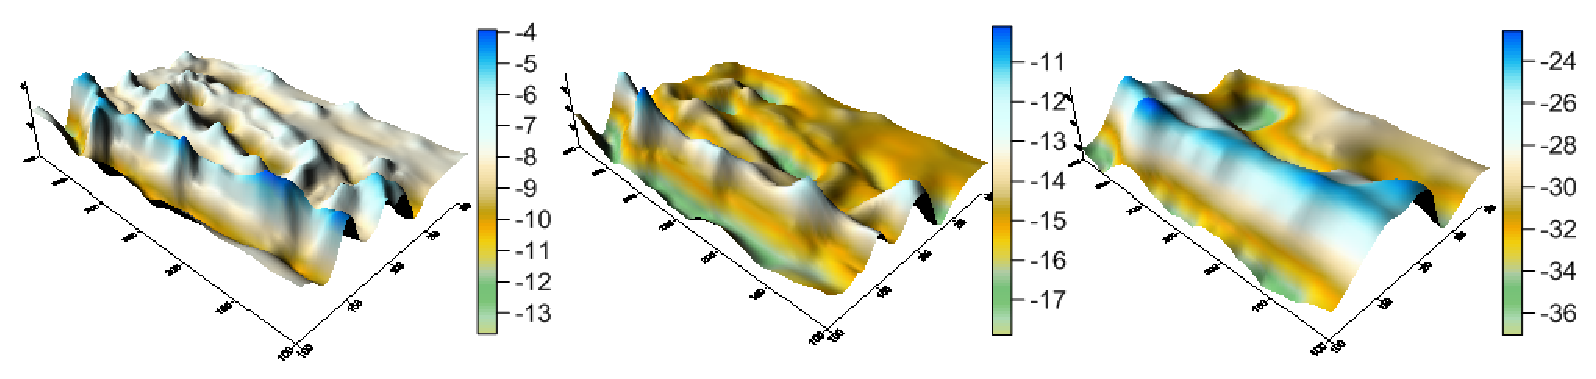
\includegraphics[height=0.2\textheight]{exact_hor}
		
		\centering\textit{Точные решения $u_0(x,y)$, $u_1(x,y)$, $u_2(x,y)$.}
	\end{figure}
	
	$H_1=8$ км, $H_2=15$ км и $H_3=30$ км. Скачки плотности $\Delta\sigma_1=0.2$ г/см$^3$, $\Delta\sigma_2=0.1$ г/см$^3$, $\Delta\sigma_3=0.1$ г/см$^3$. Шаги сетки $\Delta x=2$ км, $\Delta y=3$ км.
\end{frame}
%\begin{frame}
%	\begin{figure}
%		\centering
%		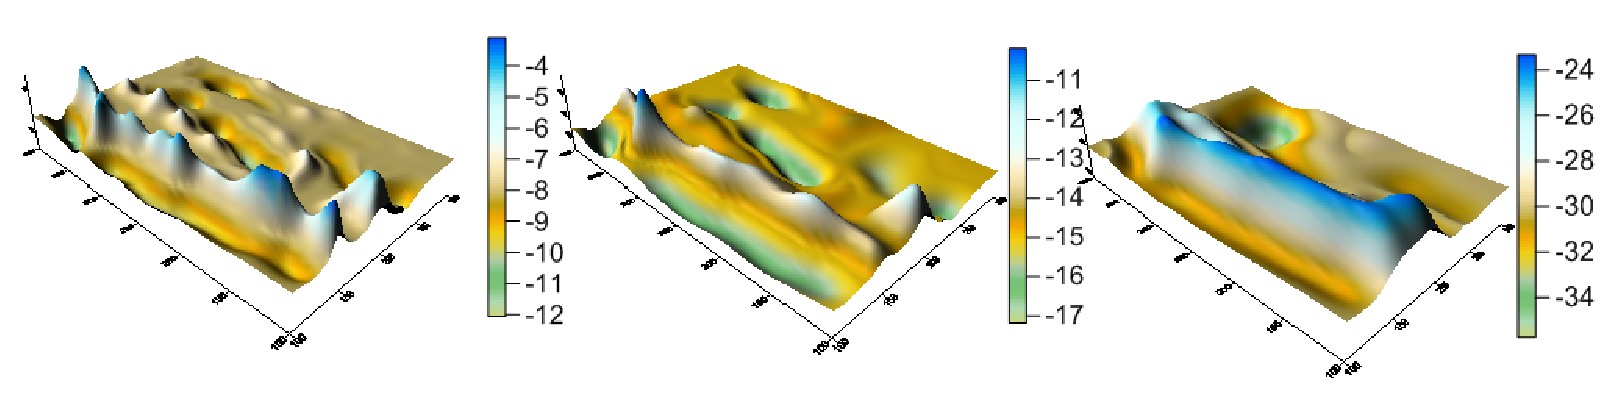
\includegraphics[height=0.2\textheight]{levmar}
%	\end{figure}
%	\centering\textit{Границы, восстановленные ЛМ $\tilde{u}_0(x,y)$, $\tilde{u}_1(x,y)$, $\tilde{u}_2(x,y)$.}
%	\begin{figure}
%		\centering
%		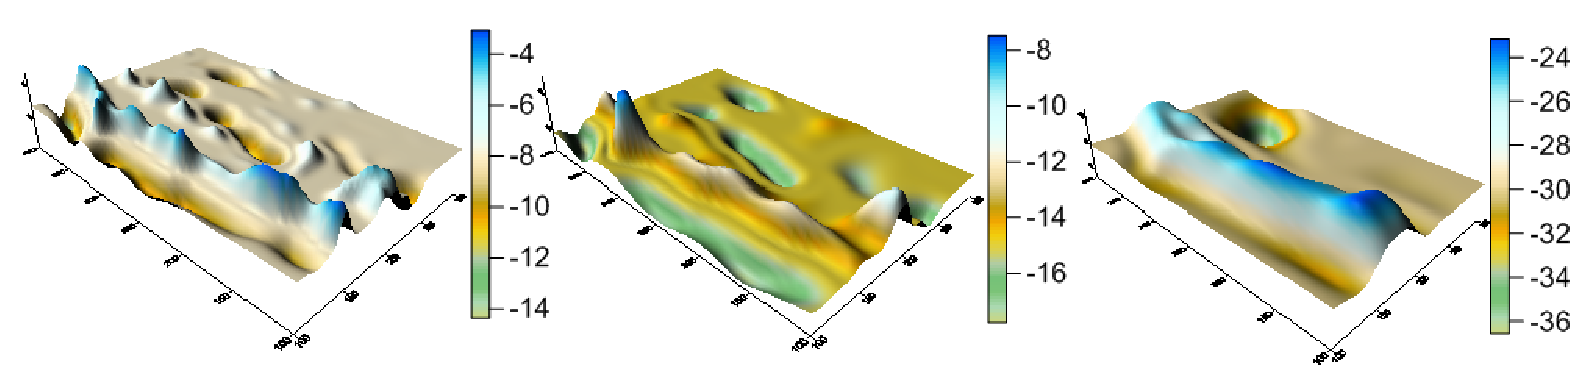
\includegraphics[height=0.2\textheight]{clm}
%	\end{figure}
%	\centering\textit{Границы, восстановленные ПЛМ $\hat{u}_0(x,y)$, $\hat{u}_1(x,y)$, $\hat{u}_2(x,y)$.}
%\end{frame}
%\begin{frame}
%	\begin{figure}
%		\centering
%		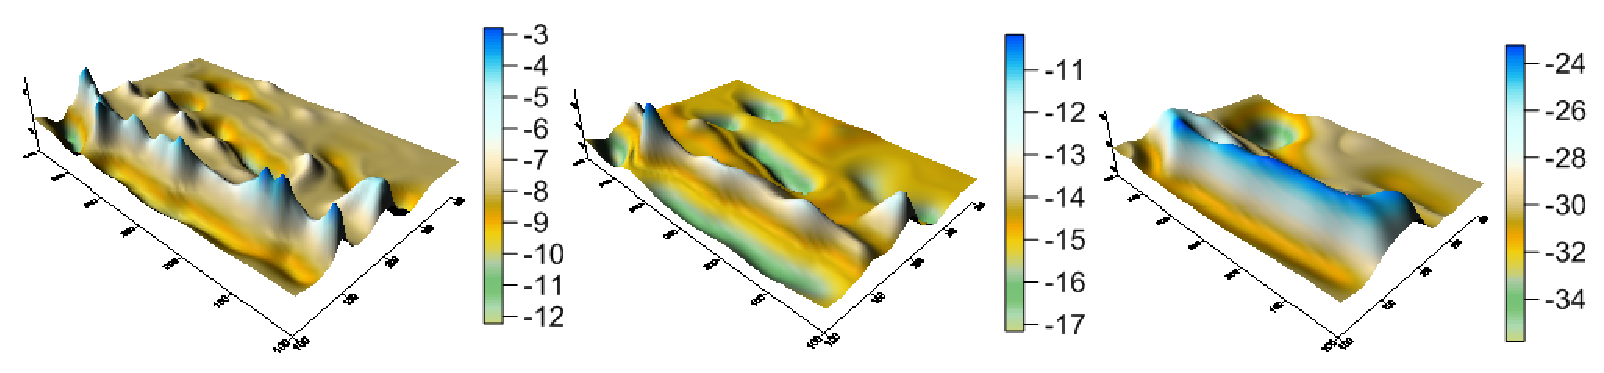
\includegraphics[height=0.2\textheight]{lm_noise}
%	\end{figure}
%	\centering\textit{Границы, восстановленные ЛМ для данных с шумом $\tilde{u}_0(x,y)$, $\tilde{u}_1(x,y)$, $\tilde{u}_2(x,y)$.}
%	\begin{figure}
%		\centering
%		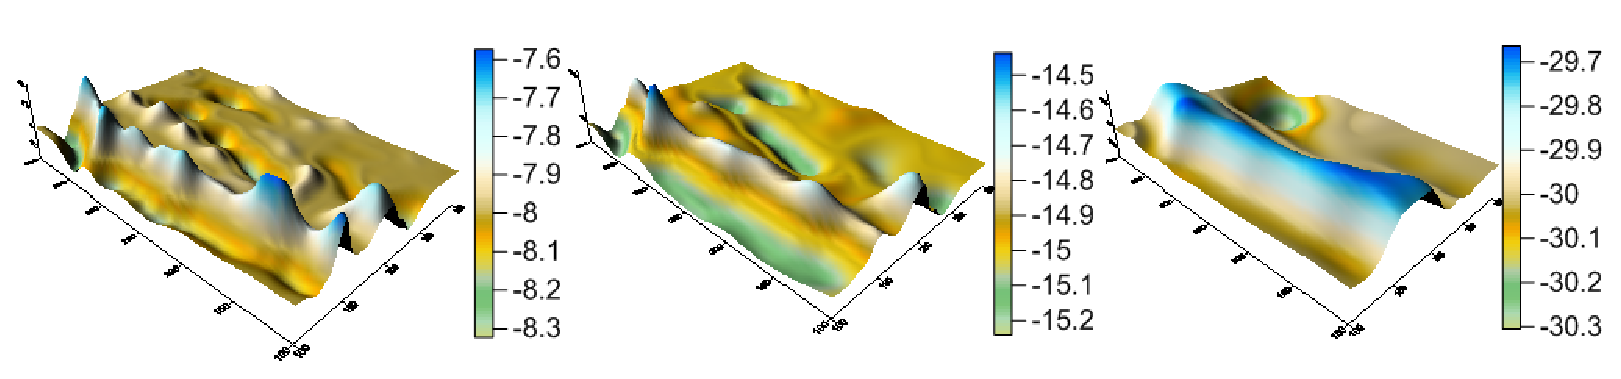
\includegraphics[height=0.2\textheight]{clm_noise}
%	\end{figure}
%	\centering\textit{Границы, восстановленные ПЛМ для данных с шумом $\hat{u}_0(x,y)$, $\hat{u}_1(x,y)$, $\hat{u}_2(x,y)$.}
%\end{frame}
\begin{frame}
	\begin{itemize}
		\item сетка $1000\times1000$,
		\item параметр регуляризации $\alpha=10^{-3}$ и демпфирующий множитель $\gamma=1$,
		\item $\varepsilon=\frac{\|A(u_a)+\alpha u_a-f_\delta\|}{\|f_\delta\|}|=0.1$,
		\item относительные погрешности $\delta_i=\|u_a-u_e\|/\|u_e\|$,
		\item $T_1$ --- Intel Xeon (1 ядро), $T_8$ --- Intel Xeon (8 ядер),	
		\item $T_{\textup{GPU}}$ --- NVIDIA Tesla M2050.
	\end{itemize}
	\begin{table} 
		\centering
		\renewcommand{\arraystretch}{1.5} 
		{\scriptsize Табл.7. Результаты расчетов в задаче гравиметрии в многослойной среде}
		\small
\begin{tabular}{|c|c|c|c|c|c|c|c|}
\hline
\multirow{2}{*}{Метод} & \multirow{2}{*}{$N$} & \multirow{2}{*}{$\delta_1$} & \multirow{2}{*}{$\delta_2$} & \multirow{2}{*}{$\delta_3$} & \multirow{2}{*}{$T_1$} & \multirow{2}{*}{$T_8$} & \multirow{2}{*}{$T_{\textup{GPU}}$} \\
                       &                      &                             &                             &                             &                        &                        &                                     \\ \hline
ЛМ                     & 60                   & 0.052                       & 0.026                       & 0.051                       & 11.7 часа                & 1.4 часа                 & 35 мин.                             \\ \hline
\rowcolor{Green}
ПЛМ                    & 20                   & 0.051                       & 0.035                       & 0.06                        & 1.2 часа                 & 10 мин.                & 3 мин.                              \\ \hline
\end{tabular}
	\end{table}
\end{frame}
\begin{frame}{}
	Параметр шага $\gamma=1$, параметры регуляризации $\alpha=0.1$, $\bar{\alpha}=1$, критерий останова $\Delta=\|A(u^k)+\alpha(u^k-u^0)-f_\delta\|/\|f_\delta\|<0.15$.
	\begin{table}[H]
		\centering
		{\scriptsize Табл.8. Относительные ошибки для задачи с шумом}
		\begin{tabular}{|l|c|l|l|l|}
			\hline
			\textbf{Метод} & \textbf{$N$} & \textbf{$\delta_1$} & \textbf{$\delta_2$} & \textbf{$\delta_3$} \\ \hline
			ЛМ                                                    & 24                            & 0.048                                & 0.035                                & 0.059                                \\ \hline
			ПЛМ                                                   & 8                             & 0.048                                & 0.040                                & 0.068                                \\ \hline
		\end{tabular}
	\end{table}
	\textbf{\color{blue}Вывод:} решения, полученные двумя методами, близки между собой и близки к истинному решению. Покомпонентный метод Левенберга -- Марквардта решает задачу в 10 раз быстрее.
	%использование
	покомпонентного метода типа Левенберга – Марквардта позволяет избежать трудностей, возникающих при применении классического метода Левенберга – Марквардта: обращение плохо обусловленных матриц, высокая вычислительная сложность и большие затраты памяти. Результаты численного моделирования показывают, что относительная норма невязки покомпонентного метода сходится
	к $\Delta$ за меньшее число итераций, чем классический регуляризованный метод Левенберга – Марквардта.
\end{frame}

\begin{frame}{Основные результаты}
	1. Для нелинейного уравнения с монотонным оператором доказаны теоремы о сходимости регуляризованного метода Ньютона. 
	Построены нелинейные аналоги $\alpha$-процессов:  регуляризованные методы градиентного типа для решения нелинейного уравнения с монотонным оператором: метод минимальной ошибки, метод наискорейшего спуска, метод минимальных невязок. Доказаны теоремы сходимости и сильная фейеровость итерационных процессов. Для задачи с немонотонным оператором, производная которого имеет неотрицательный спектр, доказаны теоремы сходимости для метода  Ньютона, нелинейных $\alpha$-процессов и их модифицированных вариантов.
	  
	
\end{frame}

\begin{frame}{Основные результаты}
	2. Для решения систем нелинейных интегральных уравнений с 
	ядром оператора структурной обратной задачи гравиметрии для 
	модели двухслойной среды предложен покомпонентный метод 
	типа Ньютона. Предложена вычислительная оптимизация метода 
	Ньютона и его модифицированного варианта при решении задач 
	с матрицей производной, близкой к ленточной. Для решения систем 
	нелинейных уравнений структурных обратных задач гравиметрии 
	для модели многослойной среды предложен покомпонентный
	метод типа Левенберга – Марквардта с весовыми множителями.
	При решении модельных обратных задач гравиметри на больших 
	сетках продемонстрирована экономичность предложенных методов
	по вычислениям и затратам оперативной памяти.
	
	3. Разработан комплекс параллельных программ для многоядерных и графических процессоров (видеокарт) решения обратных задач гравиметрии и магнитометрии на сетках большой размерности методами Ньютоновского типа и покомпонентными методами. 
\end{frame}
	
\begin{frame}{Апробация работы}
	Основные результаты по материалам диссертационной работы докладывались на конференциях:
	
	
	1. XIV и XV Уральская молодежная научная школа по геофизике (Пермь, 2013 г., Екатеринбург 2014 г.);
	
	2. Международная коференция "Параллельные вычислительные технологии" (Ростов-на-Дону, 2014 г., Екатеринбург, 2015 г., Казань, 2017 г.);
	
	3. Международная конференция "Геоинформатика: теоретические и прикладные аспекты" (Киев 2014, 2015, 2016 г.)
	
	4. Международная конференция "Актуальные проблемы вычислительной и прикладной математики" (Новосибирск, 2014 г.)
	
	5. Международный научный семинар по обратным и некорректно поставленным задачам (Москва, 2015 г.)
\end{frame}

\begin{frame}{Публикации ВАК}
\scriptsize
	\begin{enumerate}
		\item Васин В.В., Скурыдина, А.Ф. Двухэтапный метод построения регуляризующих алгоритмов для нелинейных некорректных задач // Труды ИММ УрО РАН Т.23 В.1 (2017), С. 57–74.
		\item Васин В.В., Акимова Е.Н., Миниахметова А.Ф. Итерационные алгоритмы ньютоновского типа и их приложения к обратной задаче гравиметрии // Вестник ЮУрГУ. Т.6 В.3 (2013), С. 26–37.
		\item Акимова Е. Н., Мисилов В. Е., Скурыдина А. Ф. Параллельные алгоритмы решения структурной обратной задачи магнитометрии на МВС // Вестник УГАТУ. 2014. Т.18, № 4 (65). C. 206-215.
		\item Skurydina A. F. Regularized Levenberg –- Marquardt Type Method Applied to the Structural 
Inverse Gravity Problem in a Multilayer Medium and its Parallel Realization // Bulletin of South Ural State University.
 Series: Computational Mathematics and Software Engineering. 2017. V.6, N.3. pp. 5--15.
		\item Акимова, Е. Н., Мисилов, В. Е., Скурыдина, А. Ф., Третьяков, А. И. Градиентные методы решения структурных обратных задач гравиметрии и магнитометрии 	на суперкомпьютере “Уран” // Вычислительные методы и программирование, 2015. Т. 16, 155–164.
	\end{enumerate}
\end{frame}
\begin{frame}{Публикации SCOPUS}
\scriptsize
	\begin{enumerate}
		\setcounter{enumi}{5}
		\item Akimova E., Miniakhmetova A., Martyshko M. Optimization and parallelization of Newton type methods for solving structurial gravimetry and magnetometry inverse problems // EAGE Geoinformatics 2014 – 13th Intern. Conference on Geoinformatics – Theoretical and Applied Aspects. Kiev, Ukraine. 12–15 May 2014
		\item Akimova E., Skurydina A. A componentwise Newton type method for solving the structural inverse gravity problem // EAGE Geoinformatics 2015 – 14th Intern. Conference on Geoinformatics – Theoretical and Applied Aspects. Kiev, Ukraine. 11–14 May 2015.
		\item Akimova E., Skurydina A. On solving the three-dimensional structural gravity problem for the case of a multilayered medium by the componentwize Levenberg-Marquardt method // EAGE Geoinformatics 2016 – 15th Intern. Conference on Geoinformatics – Theoretical and Applied Aspects. Kiev, Ukraine. 10–13 May 2016.
	\end{enumerate}
\end{frame}
\begin{frame}{Другие публикации}
	\begin{enumerate}
		\setcounter{enumi}{8}
			\item Мисилов В.Е., Миниахметова А.Ф., Дергачев Е.А. Решение обратной задачи гравиметрии итерационными методами на суперкомпьютере «Уран» // Труды XIV Уральской молодежной научной школы по геофизике. Пермь:
			ГИ УрО РАН.  2013. С. 187–190
			\item Миниахметова А.Ф. Сравнение быстрых методов решения структурной обратной задачи магнитометрии // Труды XV Уральской молодежной научной школы по геофизике. Екатеринбург: ИГФ УрО РАН. 2014. С.~160–162
			\item E. N. Akimova, A. F. Miniakhmetova, V. E. Misilov. Fast stable parallel algorithms for solving gravimetry and magnetometry inverse problems // The International conference "Advanced mathematics, computations and applications – 2014". Institute of Computational Mathematics and Mathematical Geophysics of Siberian Branch of RAS, Novosibirsk, Russia. June 8–11, 2014.
	\end{enumerate}
\end{frame}
\begin{frame}{Другие публикации}
	\begin{enumerate}
		\setcounter{enumi}{10}
		\item Акимова Е.Н., Мисилов В.Е., Миниахметова А.Ф. Параллельные алгоритмы решения структурной обратной задачи магнитометрии на многопроцессорных вычислительных системах  // Труды межд. конференции «Параллельные вычислительные технологии (ПАВТ’2014)», Ростов-на-Дону, 31 мар. – 4 апр. 2014 г. Челябинск:  ЮУрГУ. 2014. С. 19–29.
		\item В.В. Васин, А.Ф. Скурыдина. Регуляризованные модифицированные процессы градиентного типа для нелинейных обратных задач // Международный научный семинар по обратным и некорректно поставленным задачам. Москва, 19 – 21 ноября 2015 г.
		\item Акимова, Е. Н., Мисилов, В. Е., Скурыдина, А. Ф., Третьяков, А. И. Градиентные методы решения структурных обратных задач гравиметрии и магнитометрии на суперкомпьютере “Уран” // Труды межд. конференции «Параллельные вычислительные технологии (ПАВТ’2015)», Екатеринбург, 31 мар. – 2 апр. 2015 г. Челябинск: ЮУрГУ.  2015. С. 8–18.
	\end{enumerate}
\end{frame}

\begin{frame}\label{lastpage}
	\Huge{\centerline{Спасибо за внимание!}}
\end{frame}

%\begin{frame}
%	\begin{block}{\bf Теорема ~2.1.} 
%		Пусть $A$ --- монотонный оператор, для которого выполнены условия 
%		$$\|A(u)-A(v)\|\leqslant N_1\|u-v\|, \quad \forall u, v \in U,$$ 
%		$$\|A'(u)-A'(v)\|\leqslant N_2\|u-v\|, \quad \forall u, v \in U,$$
%		известна оценка для нормы производной в точке $u^0$, т.е.
%		$$	\|A'(u^0)\| \leqslant N_0\leqslant N_1, \quad \|u^0-u_\alpha\| \leqslant r \quad
%		u^0 \in S_r(u_\alpha),$$ $$r\leqslant \alpha/N_2, \quad 0<\alpha \leqslant \bar\alpha.$$ 
%		
%		\smallskip
%		Тогда для процесса (2.1) c $\gamma=1$ имеет место линейная скорость сходимости метода при аппроксимации единственного решения $u_\alpha$ регуляризованного уравнения (1.2)
%		$$\| u^{k}-u_\alpha \| \leqslant q^kr, \quad q=(1-\frac{\alpha}{2\bar\alpha}).$$
%	\end{block}
%\end{frame}
%\begin{frame}
%	\begin{block}{\bf Теорема ~2.2.}
%		Пусть для монотонного оператора $A$ выполнены условия $$
%		\|A(u)-A(v)\|\leqslant N_1\|u-v\|,
%		\|A'(u)-A'(v)\|\leqslant N_2\|u-v\|, \quad \forall u, v \in U,$$
%		$$\|A'(u^0)\| \leqslant N_0\leqslant N_1, \quad \|u^0-u_\alpha\| \leqslant r, $$
%		\smallskip
%		$A'(u^0)$ --- самосопряженный оператор, $\|u_\alpha-u^0\|\leqslant r \quad  
%		0\leqslant\alpha\leqslant\bar\alpha,\quad\bar\alpha\geqslant 4N_1,\quad r\leqslant\alpha/8N_2.$
%		\vspace{3mm}
%		
%		Тогда для оператора
%		$$ F(u)=(A'(u)+\bar\alpha I)^{-1}(A(u)+\alpha(u-u^0)-f_\delta) $$
%		справедлива оценка снизу
%		$$<F(u), u-u_\alpha>\geqslant\frac{\alpha}{4\bar\alpha}{\|u-u_\alpha\|}^2 \quad \forall u \in S_r(u_\alpha).$$
%	\end{block}
%\end{frame} 
%\begin{frame}
%	\begin{block}{\bf Теорема ~2.3.}
%		Пусть выполнены условия теоремы 2.2. Тогда при
%		$\gamma<\frac{\alpha\bar\alpha}{2(N_1+\alpha)^2}$
%		оператор шага $T$ процесса (2.1) при
%		$$\nu=\frac{\alpha\bar\alpha}{2\gamma(N_1+\alpha)^2}-1$$
%		удовлетворяет неравенству (2.3), для итераций $u^k$ справедливо соотношение (2.4) и имеет место сходимость
%		$$\lim_{k\to\infty}\|u^k-u_\alpha\|=0.$$
%		Если параметр $\gamma$ принимает значение ${\gamma}_{opt}=\frac{\alpha\bar\alpha}{4(N_1+\alpha)^2},$ то справедлива оценка $$\|u^k-u_\alpha\|\leqslant q^k r, \quad q=\sqrt{1-\frac{{\alpha}^2}  {16(N_1+\alpha)^2}}.$$
%	\end{block}
%\end{frame}
%\begin{frame}{3.2. Сходимость нелинейных $\alpha$-процессов}
%	\begin{block}{\bf Теорема ~3.1.}
%		Пусть для монотонного оператора $A$ выполнены условия $$\|A'(u)-A'(v)\|\leqslant N_2\|u-v\|, \quad \forall u, v \in U,	$$$$\|A'(u^0)\| \leqslant N_0\leqslant N_1, \quad \|u^0-u_\alpha\| \leqslant r,$$ и $A'(u^0)$ --- самосопряженный оператор. 
%		
%		Кроме того, для ММО параметры $\alpha$, $\bar\alpha$, $r$, $N_2$, $N_0$ удовлетворяют дополнительным соотношениям:
%		$$\alpha \leqslant \bar\alpha, \quad r\leqslant \alpha/8N_2, \quad \bar\alpha \geqslant N_0.$$
%		
%		Тогда справедливы соотношения
%		$$\|F^\varkappa(u)\|^2 \leqslant \mu_\varkappa<F^\varkappa(u), u-u_\alpha>, \quad \varkappa=-1,0,1,$$ где
%		$$
%		\mu _{-1}=\frac{4(N_1+\alpha)^2}{\alpha\bar\alpha}, \quad \mu _0= \frac{(N_1+\alpha)^2(N_1+\bar\alpha)}{\alpha{\bar\alpha}^2}, $$$$\quad \mu_1= \frac{(N_1+\alpha)^2(N_1+\bar\alpha)^2}{\alpha{\bar\alpha}^3},
%		$$
%		соответственно для ММО, МНС, ММН.
%	\end{block}
%\end{frame}
%\begin{frame}
%	\begin{block}{\bf Теорема ~3.2.}
%		Пусть выполнены условия теоремы 3.1. Тогда при
%		$$\gamma _\varkappa <\frac{2}{\mu _\varkappa}\quad (\varkappa=-1,0,1)$$
%		для последовательности $\{u^k\}$, порождаемой $\alpha$-процессом при соответствующем $\varkappa$, имеет место сходимость $$\lim_{k\to\infty}\|u^k-u_\alpha\|=0, $$ а при 
%		$\gamma{_\varkappa^{opt}}=\frac{1}{\mu_\varkappa}$
%		справедлива оценка $\|u^k-u_\alpha\|\leqslant q{_\varkappa^k}r,$ где
%		$$
%		q_{-1}=\sqrt{1-\frac{\alpha^2}{16(N_1+\alpha)^2}}, \quad q_0=\sqrt{1-\frac{\alpha^2\bar\alpha^2}{(N_1+\alpha)^2(N_1+\bar\alpha)^2}}, \quad $$$$q_1=\sqrt{1-\frac{\alpha^2\bar\alpha^4}{(N_1+\bar\alpha)^4}}.
%		$$
%	\end{block}
%\end{frame}
%\begin{frame}{\small\textbf{Случай монотонного оператора уравнения}}
%	\begin{block}{Теорема 3.5}
%		Пусть выполнены условия $$\|A(u)-A(v)\|\leqslant N_1\|u-v\|,  \quad \forall u, v \in U,$$ 
%		%$$\|A'(u)-A'(v)\|\leqslant N_2\|u-v\|, \quad \forall u, v \in U,$$
%		$$\|A'(u^0)\| \leqslant N_0, \quad \|u^0-u_\alpha\| \leqslant r,$$ 
%		
%		\smallskip
%		Оператор $A$ монотонный, $A'(u^0)$ --- самосопряженный оператор.
%		
%		\smallskip
%		Тогда при $$\gamma=\frac{2\alpha^3}{(N_0+\alpha)(N_1+\alpha)^2}$$ каждая из последовательностей, порождаемых процессами (3.3)-(3.5) сходится к регуляризованному решению $u_\alpha$ и удовлетворяет свойству Фейера.
%		Для $$\gamma=\frac{\alpha^3}{(N_0+\alpha)(N_1+\alpha)^2}$$ справедлива оценка
%		$$\|u^k-u_\alpha\|\leqslant q^k r,$$ где
%		$$q=\sqrt{1-\frac{\alpha^4}{(N_0+\alpha)^2(N_1+\alpha)^2}}.$$
%	\end{block}
%\end{frame}
%\begin{frame}{4. Оценка погрешности двухэтапного метода}
%	Согласно \textbf{\color{red}(Tautenhahn, 2002)}, при условии монотонности оператора и истокообразной представимости решения $\hat{u}$ уравнения (1.1)
%	$$u^0-\hat{u}=A'(\hat{u})v,\eqno (4.1)$$
%	справедлива оценка погрешности регуляризованного решения
%	$$\|u_\alpha^{\delta}-\hat{u}\|\leqslant\|u_\alpha^{\delta}-u_\alpha\|+\|u_\alpha-\hat{u}\|\leqslant\frac{\delta}{\alpha}+k_0\alpha,
%	\eqno (4.2)$$
%	где $k_0=(1+N_2\|v\|/2)\|v\|$, $u_\alpha^{\delta}$, $u_\alpha$ --- решения уравнения (1.2) с возмущенной $f_\delta$ и точной $f$ правой частью уравнения (1.1) соответственно. 
%	
%	Минимизируя правую часть соотношения (4.2) по $\alpha$, имеем $\alpha(\delta)=\sqrt{\delta /k_0}$, что дает оценку
%	$$\|u_{\alpha(\delta)}^{\delta, k}-\hat{u}\|\leqslant 2\sqrt{\delta k_0} \eqno (4.3)$$
%	Для итерационных процессов РМН, ММО, МНС, ММН получены оценки вида 
%	$$\|u_{\alpha(\delta)}^{\delta, k}-u_{\alpha(\delta)}^{\delta}\|\leqslant q^{k}(\delta)r \eqno (4.4)$$
%\end{frame}
%\begin{frame}{4.1. Оценка погрешности в случае монотонного оператора}
%	Объединяя оценки (4.3), (4.4), приходим к следующему утверждению
%	\begin{block}{\bf Теорема~4.1.}
%		Пусть для решения $\hat{u}$ уравнения (1.1) с монотонным оператором справедливо условие (4.1) и для метода (3.1) выполнены условия теоремы (3.1). Тогда при выборе числа итераций по правилу
%		$$ k(\delta)=\left[\frac{\ln(2\sqrt{k_0\delta}/r)}{\ln q(\delta)}\right]$$
%		справедлива оптимальная по порядку оценка погрешности двухэтапного метода
%		$$ \|u_{\alpha(\delta)}^{\delta, k}-u_{\alpha(\delta)}^{\delta}\|\leqslant 4\sqrt{k_0 \delta}.$$
%	\end{block}
%	\let\thefootnote\relax\let\thefootnote\relax\footnotetext{\footnotesize В. В. Васин В.В., Скурыдина, А.Ф. Двухэтапный метод построения регуляризующих алгоритмов для нелинейных некорректных задач // Труды ИММ УрО РАН Т.23 В.1 (2017), С. 57–74.}
%\end{frame}
%\begin{frame}{4.2. Оценка погрешности в случае оператора c положительным спектром}
%	В этой ситуации для двухэтапного алгоритма можно установить оценку для невязки --- основной характеристики точности метода при решении задачи с реальными данными.
%	Пусть регуляризованное уравнение разрешимо, тогда для его решения $u_{\alpha(\delta)}^{\delta}$ справедливо соотношение
%	$$\|A(u_{\alpha(\delta)}^{\delta})-f_\delta\|=\alpha\|u_{\alpha(\delta)}^{\delta}-u^0\|.\eqno (4.5)$$
%	Пусть для некоторой связи $\alpha(\delta)$ $\|u_{\alpha(\delta)}^{\delta}-u^0\|\leqslant m <\infty$, что влечет оценку
%	$$\|A(u_{\alpha(\delta)}^{\delta})-f_\delta\|\leqslant\alpha(\delta)m \eqno (4.6)$$
%	и сходимость $$\lim_{\delta\to 0}\|A(u_{\alpha(\delta)}^{\delta})-f_\delta\|=0,$$ при $\alpha(\delta)\to 0$, $\delta\to 0$.
%	\let\thefootnote\relax\let\thefootnote\relax\footnotetext{\footnotesize В. В. Васин В.В., Скурыдина, А.Ф. Двухэтапный метод построения регуляризующих алгоритмов для нелинейных некорректных задач // Труды ИММ УрО РАН Т.23 В.1 (2017), С. 57–74.}
%\end{frame}
%\begin{frame}
%	Пусть ${u_{\alpha(\delta)}^{\delta, k}}$ --- итерационные точки, полученные одним из методов рассмотренных выше методов. Имеем
%	$$\|A(u_{\alpha(\delta)}^{\delta, k})-f_\delta\|\leqslant\|A(u_{\alpha(\delta)}^{\delta, k})-A(u_{\alpha(\delta)}^{\delta})\|+\|A(u_{\alpha(\delta)}^{\delta})-f(\delta)\|\leqslant N_1 r q^{k(\delta)}+\alpha(\delta)m.
%	\eqno (4.7)$$
%	Выбирая, например, $\alpha(\delta)=\delta^p$ и приравнивая слагаемые в правой части (4.7), получаем правило выбора числа итерации
%	$$k(\delta)=\left [\ln(m\delta^p/N)/\ln q(\delta)\right ],$$
%	при котором справедлива оценка для невязки двухэтапного метода
%	$$\|A(u_{\alpha(\delta)}^{\delta})-f_\delta\|=2m\delta^p.\eqno (4.8)$$
%	\begin{block}{Замечание~4.3} Соотношения (4.5)---(4.8) остаются справедливыми для случая, когда матрицы $A'(u^k)$ содержат набор малых отрицательных собственных значений с тем лишь отличием, что в неравенстве (4.7) параметр $q$ во всех методах теперь вычисляется по формулам из раздела 3, в которых параметр $\bar\alpha$ заменен на $\alpha^*$ (см. замечание 3.2).
%	\end{block}
%	\let\thefootnote\relax\let\thefootnote\relax\footnotetext{\footnotesize В. В. Васин В.В., Скурыдина, А.Ф. Двухэтапный метод построения регуляризующих алгоритмов для нелинейных некорректных задач // Труды ИММ УрО РАН Т.23 В.1 (2017), С. 57–74.}
%\end{frame}
%\begin{frame}{1.2. Нелинейные аналоги альфа-процессов \textbf{(new)}}
%	Альфа-процессы для линейного  самосопряженного положительно определенного оператора  были предложены {\color{red}М.~А.~Красносельским и др. (1969)}. \\
%	Для нелинейного оператора итерационный процесс запишем в виде:
%	$$u^{k+1}=u^k-\beta_k(A(u^k)-f_{\delta}).$$ \\
%	Выбирая параметр $\beta_k$ из условия
%	$$\min_{\beta_k}{\|u^k-\beta_k(A(u^k)-f_{\delta})-z\|^2},$$ где $z$ --- решение уравнения $A'(u^k)z=y^k$, $y^k=f_{\delta}+A'(u^k)u^k-A(u^k)$ (используем разложение Тейлора в точке $u^k$), получим {\color{blue} регуляризованный метод минимальной ошибки (ММО)}
%	$$u^{k+1} =u^k - \frac{\langle B^{-1}(u^k)S_\alpha(u^k), S_\alpha (u^k)\rangle}{\|S_\alpha(u^k)\|^2}S_\alpha(u^k),$$ где $B(u^k)=A'(u^k)+\bar{\alpha}I, \quad S_\alpha(u^k)=A(u^k)+\alpha(u^k-u^0)-f_\delta$.
%\end{frame}
%\begin{frame}
%	Если использовать экстремальные принципы
%	$$\min_{\beta_k}\{\langle A'(u^k)u^{k+1},u^{k+1}\rangle-2\langle u^{k+1},y^k\rangle\},$$
%	либо
%	$$\min_{\beta_k}\{\|A'(u^k)(u^k-\beta_k(A(u^k)-f_{\delta})-y^k\|^2\},$$
%	то получаем нелинейные {\color{blue}регуляризованные методы наискорейшего спуска (МНС)}
%	$$u^{k+1} =u^k - \frac{\langle S_\alpha(u^k), S_\alpha (u^k)\rangle}{\langle B(u^k)S_\alpha(u^k), S_\alpha(u^k)\rangle}(A(u^k)+\alpha(u^k-u^0)-f_\delta)$$
%	и {\color{blue}минимальных невязок (ММН)}
%	$$u^{k+1} =u^k - \frac{\langle B(u^k)S_\alpha(u^k), S_\alpha (u^k)\rangle}{\|B(u^k)S_\alpha(u^k)\|^2}(A(u^k)+\alpha(u^k-u^0)-f_\delta).$$
%	
%	\smallskip
%	В общем виде итерационную последовательность обозначим
%	$$ u^{k+1}=u^k-\gamma\frac{\langle(A'(u^k)+\bar\alpha I)^{\varkappa}S_\alpha(u^k), S_\alpha(u^k)\rangle}{\langle(A'(u^k)+\bar\alpha I)^{\varkappa+1}S_\alpha(u^k), S_\alpha(u^k)\rangle}S_\alpha(u^k)\equiv{T(u^k)}\eqno (1.6)$$
%	при соответствующем $\varkappa=-1,0,1$, $\gamma$ --- демпфирующий множитель.
%\end{frame}
\end{document}